\documentclass[11pt]{article}

\usepackage{fancybox}


\usepackage{color}
\usepackage{url}
\usepackage[margin=1in]{geometry}
\usepackage{setspace}
\usepackage{lscape}
\usepackage{afterpage}

\setlength{\parskip}{1em}%
\setlength\parindent{0pt}
\renewcommand{\textfraction}{0.0}
\renewcommand{\topfraction}{1.0}
%\renewcommand{\textfloatsep}{5mm}

\usepackage{comment}
% Definitions of handy macros can go here
\usepackage{amsmath,amssymb,amsthm,bm,mathtools}
\usepackage{multirow}
\usepackage{extarrows}
\usepackage{dsfont,multirow,setspace,natbib,enumerate}
%\usepackage{dsfont,multirow,hyperref,setspace,enumerate}
%\hypersetup{colorlinks,linkcolor={blue},citecolor={blue},urlcolor={red}} 
\usepackage{algpseudocode,algorithm}
\algnewcommand\algorithmicinput{\textbf{Input:}}
\algnewcommand\algorithmicoutput{\textbf{Output:}}
\algnewcommand\INPUT{\item[\algorithmicinput]}
\algnewcommand\OUTPUT{\item[\algorithmicoutput]}

\newtheorem{innercustomgeneric}{\customgenericname}
\providecommand{\customgenericname}{}
\newcommand{\newcustomtheorem}[2]{%
  \newenvironment{#1}[1]
  {%
   \renewcommand\customgenericname{#2}%
   \renewcommand\theinnercustomgeneric{##1}%
   \innercustomgeneric
  }
  {\endinnercustomgeneric}
}


\theoremstyle{plain}
\newtheorem{thm}{Theorem}[section]
\newtheorem{lem}{Lemma}
\newtheorem{prop}{Proposition}
\newtheorem{pro}{Property}
\newtheorem{assumption}{Assumption}
\newtheorem{conj}{Conjecture}
\newcustomtheorem{customthm}{Theorem}
\newcustomtheorem{customlem}{Lemma}
\newcustomtheorem{customconj}{Conjecture}
\newcustomtheorem{customrmk}{Remark}

\theoremstyle{definition}
\newtheorem{defn}{Definition}
\newtheorem{cor}{Corollary}
\newtheorem{example}{Example}
\newtheorem{rmk}{Remark}


\setcounter{figure}{0}   
\setcounter{table}{0}  



\newcommand{\of}[1]{\left(#1\right)}
\newcommand{\off}[1]{\left[#1\right]}
\newcommand{\offf}[1]{\left\{#1\right\}}
\newcommand{\aabs}[1]{\left|#1\right|}



%\usepackage{xcolor}

\newcommand{\cmt}[1]{{\leavevmode\color{red}{#1}}}


\usepackage{dsfont}
\usepackage{multirow}

\DeclareMathOperator*{\minimize}{minimize}


\usepackage{mathtools}
\mathtoolsset{showonlyrefs}
\newcommand*{\KeepStyleUnderBrace}[1]{%f
  \mathop{%
    \mathchoice
    {\underbrace{\displaystyle#1}}%
    {\underbrace{\textstyle#1}}%
    {\underbrace{\scriptstyle#1}}%
    {\underbrace{\scriptscriptstyle#1}}%
  }\limits
}
\usepackage{xr}
\makeatletter
\newcommand*{\addFileDependency}[1]{% argument=file name and extension
  \typeout{(#1)}
  \@addtofilelist{#1}
  \IfFileExists{#1}{}{\typeout{No file #1.}}
}
\makeatother

\newcommand*{\myexternaldocument}[1]{%
    \externaldocument{#1}%
    \addFileDependency{#1.tex}%
    \addFileDependency{#1.aux}%
}
\myexternaldocument{main3}


% adjust table separation
%\setlength{\tabcolsep}{6pt} % Default value: 6pt
%\renewcommand{\arraystretch}{1.5}

\def\fixme#1#2{\textcolor{red}[FIXME (#1): #2]}

\input macros.tex
\usepackage{mathrsfs}  
\def\caliB{\mathscr{B}}

\usepackage[english]{babel}
\usepackage[dvipsnames]{xcolor}

\usepackage{enumitem,kantlipsum}

\title{\textbf{Response Letter}}

\date{}
\author{}


\begin{document}

\maketitle
\vspace{-1.5cm}

We are grateful to the reviewers for their careful reading and thoughtful comments. Please note that the \textbf{Response to Major Comments Summarized by Editor} consists of general comments raised by both reviewers. We address these issues upfront {\bf in pages 1-7 of this letter}. 

\begin{center}
    \textbf{Response to Major Comments Summarized by Editor}
\end{center}

\begin{enumerate}[wide, labelwidth=!, labelindent=0pt]
    \item \textit{The question about whether the monotonicity assumption for the Borda count algorithm can be weaken.}
    
    \textbf{Response:}
Inspired by reviewers' comments, we have improved our results on computational limits. We add a new section 5.1 with a new Theorem 3, which roughly says:

\begin{quote}
\color{blue}
``There exists \emph{no} polynomial-time algorithm that achieves the minimax statistical bound in the general setting, under the popular computational hardness conjecture on hypergraphic planted clique (HPC) detection and some technical conditions.''
\end{quote}
The new theory has suggested the need of extra assumptions for polynomial-time algorithms. The new section reads: 
    
 
 \begin{quote}
``...We should point out that computing the least-squares optimizer $(\hat\Theta^{\text{LSE}},\hat\pi^{\text{LSE}})$ in \eqref{eq:lseopt} generally entails exponential complexity, even in the simple matrix case~\citep{gao2015rate}. {\color{blue}Specifically, in this section {\color{blue} we show the non-existence of \emph{polynomial-time algorithms} with rate~\eqref{eq:rate} under the computational hardness conjecture for hypergraphic planted clique (HPC)~\citep{luo2022tensor}. The computational limit implies the necessity of extra assumptions to achieve the optimal rate~\eqref{eq:rate} via polynomial algorithms. \\

{\bf 5.1 Computational limits under HPC detection conjecture}\\

The hypergraphic planted clique detection conjecture plays an important role in constructing the computational limits of our problem. We briefly introduce the HPC hardness conjecture. 

Consider an $m$-uniform hypergraph $G = (V,E)$, where $V$ is a set of vertices, and $E$ is a set of hyperedges. An Erd\"os-R\'enyi random hypegraph, denoted by $\tG_m(d,1/2)$, is a random $m$-uniform hypergraph with $d$ vertices and probability 1/2 for each of the hyperedge connections. The hypergraphic planted clique (HPC) with clique size $\kappa>0$, denoted by $\tG_m(d,1/2,\kappa)$, is generated from Erd\"os-R\'enyi random hypegraph in the following way. First we generate an Erd\"os-R\'enyi random hypegraph from $\tG_m(d,1/2)$. Then we independently pick $\kappa$ vertices with uniform probability from $d$ vertices. Finally, we obtain the $\tG_m(d,1/2,\kappa)$ by including only the hyperedges whose vertices all belong to the picked $\tau$ vertices. The HPC detection refers to the hypothesis testing problem, 
\begin{align}\label{eq:HPC}
    H_0\colon G\sim \tG_m(d,1/2)\quad\text{v.s.}\quad H_1\colon G\sim \tG_m(d,1/2,\kappa).
\end{align}
The earlier work \citep{luo2022tensor} presents the following hardness conjecture for testing \eqref{eq:HPC}.
\begin{conj}[HPC detection conjecture \citep{luo2022tensor}]\label{conj:1} Consider the HPC problem in \eqref{eq:HPC} and let $m\geq 2$ is be fixed integer. Suppose
\[
   \limsup_{d\rightarrow\infty} \log\kappa/\log\sqrt{d}\leq 1-\tau,\quad \text{for any }\tau >0.
   \]
Then, for any polynomial-time test sequence $\{\phi\}_d\colon G \mapsto \{0,1\}$, we have 
\[
\liminf_{d\rightarrow\infty} \left\{\mathbb{P}_{H_0}(\phi(G) = 1)+ \mathbb{P}_{H_1}(\phi(G) = 0)\right\}\geq \frac{1}{2},
\]
\end{conj}

Now we construct the computational lower bound based on Conjecture~\ref{conj:1}. 

\begin{thm}[Computational lower bound under sufficient smoothness]\label{thm:nopoly} Assume Conjecture~\ref{conj:1} holds. Define the relaxed smooth tensor class
\[
\tP_{\textup{rel}}=\{\Theta: \Theta \text{ is generated from~\eqref{eq:randommodel} with fixed latent variables $\{x_i\}_{i=1}^d$ and $f\in \tF(\alpha,L)$}\}.
\]
Consider the Gaussian tensor model~\eqref{eq:obs} with $\alpha> m/2$. Then, there exists no polynomial algorithm that achieves the statistical optimal convergence $\text{Rate}(d)$. That is, 
\begin{align}\label{eq:compthm}
\frac{1}{\textup{Rate}(d)}\inf_{\hat \Theta \textup{ Polynomial-time}}\sup_{\Theta\in\tP_{\textup{rel}}}\textup{MSE}(\hat\Theta,\Theta)\rightarrow \infty, \quad \text{as}\ d\to\infty.
\end{align}
\end{thm}
Theorem~\ref{thm:nopoly} shows the \emph{impossibility} of polynomial-time estimator to achieve the optimal statistical rate in the general model. The intuition in the proof is to show the best bound for \emph{polynomial-time} tensor estimation as $d^{-m/2}$, in the absence of extra model structures. The condition $\alpha>m/2$ is a technical assumption to facilitate the proof. 
Theorem~\ref{thm:nopoly} is not a weakness of our proposed estimator; rather, it reveals the non-avoidable statistical-computational gap as a nature of the smooth tensor estimation problem. The fact has motivated us to introduce extra model structure to fill the gap.\\

{\bf 5.2 Borda count algorithm}\\

The earlier section has shown the impossibility of polynomial-time algorithms in the general model. In this section, we restrict ourself to a sub-model with extra monotonicity structures; this structure makes polynomial-time algorithm possible.} We introduce a notion of marginal monotonicity for the generative functions.....
}
\end{quote}

We have also updated the Table 2 for fair comparison. 
 \begin{table*}[h]
    \centering
    \resizebox{\textwidth}{!}{%
    \begin{tabular}{c|@{\hskip4pt}c@{\hskip5pt}c@{\hskip4pt}c@{\hskip5pt}c@{\hskip4pt}c@{\hskip5pt}c@{\hskip4pt}c@{\hskip5pt}c@{\hskip5pt}c}
    & \citet{pananjady2022isotonic}&  \citet{balasubramanian2021nonparametric}&  \citet{li2019nearest}&\textbf{Ours} (MLE) & \textbf{Ours} (Borda count)\\
    \hline
       Model structure& monotonic & Lipschitz & Lipschitz &  $\alpha$-smooth  & $\alpha$-smooth \& monotonic\\
             Fixed grid design & $\surd$ &$\times$ & $\times$ & $\times$& $\surd$\\
     Error rate for order-$m$ tensor & \multirow{2}{*}{$d^{-1}$} & $d^{-{2m\over m+2}}$ & $d^{-\lfloor m/3\rfloor }$ & $d^{-{2m\alpha\over m+2\alpha}}\vee d^{-(m-1)}$ & $d^{-{2m\alpha\over m+2\alpha}}\vee d^{-(m-1)}$ \\
       (e.g., when $(m,\alpha)=(3,1)$) & & ($d^{-6/5}$) & $(d^{-1})$ & $(d^{-6/5})$ & $(d^{-6/5})$\\
          Minimax optimality& $\surd$  & $\times$ & $\times$ & $\surd$ & $-*$ \\
     Polynomial algorithm& $\surd$ &$\times$ & $\surd$ & $\times$& $\surd$ 
    \end{tabular}
    }
    \caption{Comparison of our results with previous work. \color{blue}For simplicity, we omit the log term in the rate. $^{*}$The optimality is achieved under extra Lipchitz monotonicity conditions. }
 \label{tab:comp}
\end{table*}


We have also added a new Appendix~\ref{sec:nopoly} for the proof of Theorem~\ref{thm:nopoly}. 
\begin{quote}
\color{blue}

{\bf C.4 Proof of Theorem~\ref{thm:nopoly}}\\

The proof of Theorem~\ref{thm:nopoly} leverages results of hypergraphic planted clique and constant higher-order clustering problems. We first briefly explain the constant higher-order clustering problems. We then prove the main result.\\

{\bf C.4.1 Constant higher-order clustering and computational lower bound} \\

Let $\mk = (k_1,\ldots,k_m)$ and $\md = (d_1,\ldots,d_m)$. We introduce the constant high-order clustering (CHC) problem~\citep{luo2022tensor}. Consider a data tensor $\tY\in\bbR^{d_1\times \cdots \times d_m}$ generated from the signal plus noise model
\begin{equation}\label{eq:gaussian}
\tY=\Theta+\tE, 
\end{equation}
where the entries in $\tE$ are i.i.d. drawn from Gaussian distribution, and the signal tensor $\Theta$ contains a constant planted structure:
\begin{align}\label{eq:chcdef}
    \Theta\in\Theta_{\text{CHC}}(\mk,\md,\lambda) :=\{\lambda'\mathds{1}_{I_1}\otimes \cdots\otimes \mathds{1}_{I_m}\colon|I_i| = k_i,\ \text{for all }i\in[m],\ \lambda' \geq \lambda\}.
\end{align}
Here $I_i\subset [d_i]$ denotes a subset of indices, $|\cdot|$ denotes the cardinality of the set, $\mathds{1}_{I_i}$ is the $d_i$-dimensional indicator vector such that $(\mathds{1}_{I_i})_j = 1$ if $j\in I_i$ and 0 otherwise. The CHC detection problem is to test the following hypothesis based on the observed tensor $\tY$, 
\begin{align}\label{eq:chct}
    H_0\colon \Theta = 0\quad\text{v.s.}\quad H_1\colon \Theta\in\Theta_{\text{CHC}}(\mk,\md,\lambda).
\end{align}

The following proposition provides the asymptotic regime for impossible polynomial-time detection of CHC under Conjecture~\ref{conj:1}. This proposition plays important role to prove our Theorem~\ref{thm:nopoly}.
 \begin{prop}[Theorem 15 in \citep{luo2022tensor}]\label{prop:CHC} 
Consider CHC detection problem in \eqref{eq:chct} in the Gaussian noise model~\eqref{eq:gaussian} under the asymptotic regime $d\rightarrow\infty$ satisfying
\begin{align}\label{eq:equal}
  d =  d_1= \cdots= d_m ,\quad
    k = k_1 = \cdots = k_m = d^\delta,\quad \lambda  = d^{-\gamma},
\end{align}with $0\leq\delta\leq1$ and $\gamma >(m\delta-m/2)\vee 0.$ Then, under Conjecture~\ref{conj:1}, for any polynomial-time test sequence $\{\phi\}_d\colon \tY\mapsto\{0,1\}$, we have
\begin{align}
    \liminf_{d\rightarrow\infty} \left\{\mathbb{P}_{\tH_0}(\phi(\tY) = 1)+ \sup_{\Theta\in\Theta_{\textup{CHC}}(\mk,\md,\lambda)}\mathbb{P}_{\Theta}(\phi(\tY) =0) \right\}\geq\frac{1}{2}.
\end{align}
\end{prop}


{\bf C.4.2 Proof of Theorem~\ref{thm:nopoly}}
 \begin{proof}[Proof of Theorem~\ref{thm:nopoly}]
 Assume that  the true signal $\Theta\in\mathbb{R}^{d\times \cdots \times d}$ has constant planted structure with a given $\mk=(k,\ldots,k)$ such that 
\begin{align}
    \Theta \in\Theta_{\text{CHC}}(\mk,\md,\lambda) = \{ \lambda \mathds{1}_{I}\otimes \cdots\otimes \mathds{1}_{I}\colon  |I| = k\}.
\end{align}
We have $\Theta_{\text{CHC}}\subset \tP_{\textup{rex}}$, because we can set the infinitely smooth function $f: [0,1]^m \to[0,1]$ by
\begin{equation}\label{eq:fun}
f(x_1,\ldots,x_m)=\lambda \prod_{i\in[m]}x_i.
\end{equation}
Then, there is one-to-one correspondence between tensors in $\Theta_{\textup{CHC}}(\mk,\md,\lambda)$ and tensors generated by the above $f$ under the choice $x_i=\mathds{1}_{i\in I}$ for all $i\in[m]$.



We consider the regime where polynomial-time solvable test is impossible based on Proposition~\ref{prop:CHC}. We set $\delta=1/2$, $k = c_1d^{\delta}$, and $\lambda = c_2d^{-\gamma}$ for any fixed $\gamma \in (0, {2\alpha -m \over m})$, so that any polynomial-time test sequence $\phi$ satisfies 
\[
 \liminf_{d\rightarrow\infty} \left\{\mathbb{P}_{\tH_0}(\phi(\tY) = 1)+\sup_{\Theta \in \Theta_{\textup{CHC}}(\mk,\md,\lambda)}\mathbb{P}_{\Theta}(\phi(\tY) =0) \right\}\geq\frac{1}{2}.
\]
The choice of $\lambda$ is possible given that $\alpha > m/2$. Notice that the choice $\lambda \lesssim O(1)$ ensures the function~\eqref{eq:fun} satisfies the definition~\eqref{eq:holder} for all $\alpha>0$. 

We prove by contradiction. Assume that there exists a hypothetical estimator $\hat\Theta$ from a polynomial-time algorithm  that attains the rate $\text{Rate}(d)$. Specifically, there exists a constant $b>0$ such that 
\begin{align}\label{eq:esterror}
   \limsup_{d\rightarrow\infty}\frac{1}{\textup{Rate}(d)} \sup_{\Theta\in\Theta_{\text{CHC}}(\mk,\md,\lambda)}\frac{1}{d^m}\mathbb{E}\FnormSize{}{\hat\Theta-\Theta}^2\leq b.
\end{align}
By Markov's inequality, the inequality~\eqref{eq:esterror} implies that, when $d$ is sufficiently large, for all $\Theta\in\Theta_{\text{CHC}}(\mk,\md,\lambda)$ and all $u>0$, we have
\begin{align}\label{eq:markov}
    \FnormSize{}{\hat\Theta-\Theta}\leq u \sqrt{\text{Rate}(d)d^{m}},
\end{align}
with probability at least $1-b/u$.
Consider the hypothesis test in \eqref{eq:chct}. We employ the following test 
\begin{align}
    \phi(\tY) = \mathds{1}(\FnormSize{}{\hat\Theta}\geq u\sqrt{\text{Rate}(d)d^m}).
\end{align}
The Type I error of the test $\phi$ is controlled by
\begin{align}
    \mathbb{P}_0(\FnormSize{}{\hat\Theta}\geq u\sqrt{\text{Rate}(d)d^m})  = \mathbb{P}_0(\FnormSize{}{\hat\Theta-\Theta}\geq u\sqrt{\text{Rate}(d)d^m}) \leq b/u.
\end{align}
For Type II error, we obtain,
\begin{align}
\sup_{\Theta\in\Theta_{\text{CHC}}(k,d,\lambda)}\mathbb{P}_\Theta(\phi(\tY) = 0) &= \sup_{\Theta\in\Theta_{\text{CHC}}(k,d,\lambda)}\mathbb{P}_\Theta(\FnormSize{}{\hat\Theta}< u \sqrt{\text{Rate}(d)d^m})\\&\leq\sup_{\Theta\in\Theta_{\text{CHC}}(k,d,\lambda)}\mathbb{P}_\Theta(\FnormSize{}{\hat\Theta-\Theta}^2> \FnormSize{}{\Theta}^2-u^2\text{Rate}(d)d^m)\\&\stackrel{(*)}{\leq}\sup_{\Theta\in\Theta_{\text{CHC}}(\mk,\md,\lambda)}\mathbb{P}_\Theta(\FnormSize{}{\hat\Theta-\Theta}^2> u^2\text{Rate}(d)d^m)\\&\stackrel{(**)}{\leq} b/u.
\end{align}
The inequality $(*)$ holds because 
\begin{align}\label{eq:regime}
    \FnormSize{}{\Theta}^2\geq \lambda^2 k^m = c_1^mc_2^2d^{{m\over 2}-\gamma} \geq 2 u^2\text{Rate}(d)d^m \asymp d^{{m\over 2}-{2\alpha-m \over m}}
\end{align}
where the last inequality is true under the regime $c_1^mc_2>2u^2$. We can always choose constants $c_1$ and $c_2$ given the value $u$. The inequality $(**)$ holds because of the statement~\eqref{eq:markov}. 
Putting Type I and II errors together, we obtain
\begin{align}
 \mathbb{P}_{\tH_0}(\phi(\tY) = 1)+ \sup_{\Theta\in\Theta_{\text{CHC}}(\mk,\md,\lambda)}\mathbb{P}_{\Theta}(\phi(\tY) =0) \leq 2b/u < 1/2,
\end{align}
for $u>4b$. This fact contradicts the Proposition~\ref{prop:CHC}.  Therefore, there is no polynomial-time $\hat\Theta$ satisfying \eqref{eq:esterror}.
\end{proof}
\end{quote}

    \item \textit{The question about whether this assumption should lead to higher convergence rates.}
    
    \textbf{Response:} 
Inspired by reviewer's comments, we have added a new Theorem~\ref{thm:mminimax} in the main paper. Our new theorem shows that the monotonicity does not lead to a higher convergence rate in many cases. 

We quote the new section here:
 \begin{quote}
{\color{blue}

``...The earlier section has shown the impossibility of polynomial-time algorithms in the general model. In this section, we restrict ourself to a sub-model with extra monotonicity structures; this structure makes polynomial-time algorithm possible.... ''\\

{\bf 5.2 Borda count algorithm}\\

``...We refer to $\tF(\alpha,L)\cap \tM(\beta)$ as the monotonic-plus-smooth function class. This class was initially proposed in previous literature of graphons. The work~\cite{chan2014consistent} proposes the Lipschitz monotonic function to facilitate the analysis of sorting-merging algorithm for matrix estimation; their setting is a special case of our Definition 2 with $(\alpha,\beta,m)=(1,1,2)$. Inspired by earlier work, we consider the similar monotonic-plus-smooth function class $\tF(\alpha,L)\cap \tM(\beta)$ under general configuration $\{(\alpha,\beta,m): \alpha>0,\ 0<\beta\min(\alpha,1)\leq 1, \ m\geq 2\}$. Note that the constraint $\beta \min(\alpha, 1) \leq 1$ is due to the natural relationship between joint smoothness and marginal smoothness. ...''\\

{\bf 5.3. Possible relaxation of monotonicity} \\

We have shown the success of our Borda count algorithm under extra marginal monotonicity. We refer to $\tF(\alpha,L)\cap \tB(\beta)$ as the monotonic-plus-smooth function class. This class was initially proposed in previous literature of graphons....\\\

We emphasize that our monotonicity assumption should be interpreted \emph{up to permutation} in light of~\eqref{eq:obs}. The permutation relaxes the extent of stringency in the monotonic assumptions. In the univariate case ($m=1$), \emph{every smooth function is monotonic-plus-smooth up to permutations.} In particular, $f\in \tF(1, L)$ implies the existence of permutation $\pi$ such that $(f\circ \pi) \in \tF(1, L)\cap \tB(1)$. The monotonicity comes for free in this case, because the descending sorting, as a permutation, does not deteriorate the 1-d smoothness. For general order~$m$, the monotonicity imposes moderate constraints on the marginal structure. We provide two examples to illustrate flexibility allowed in our models.  \\
  
 
 \begin{example}[Free monotonicity inherited from smoothness]\label{ex:free}Consider a quadratic function $f(x,y,z)=(x-0.5)^2+yz$. Although the function $f$ is non-monotonic, we can show that $f$ is nearly monotonic-plus-smooth up to permutations; i.e., $f$ can be identified by $\bar f\circ \pi$ for some permutation $\pi$ and $\bar f \in \tF(\alpha,L)\cap \tB(\beta)$ up to a negligible perturbation. See appendix~\ref{sec:ex} for the expression of $(\pi, \bar f)$. Therefore, our Borta count algorithm is applicable to $f$.  
 \end{example}
 
 
  \begin{example}[Decomposable monotonicity] Let $R\in\mathbb{N}_{+}$ be a constant, and $\{g_{r,i}(\cdot) \colon[0,1]\to \bbR\}$ be a set of 1-d smooth functions for $(r,i)\in[R]\times [m]$. Then, all decomposable smooth functions of the form 
  \[
  f(x_1,\ldots,x_m)=\sum_{r\in[R]}g_{r,1}(x_1)\cdots g_{r,m}(x_m),
  \]
are monotonic-plus-smooth up to permutations. In particular, low-rank tensors with smooth factors are also monotonic-plus-smooth up to permutations.
\end{example}

We show below that the additional monotonic assumptions do not change the minimax rate under Lipschitz (or equivalently, 1-smooth) condition. 

\begin{thm}[Statistical minimax lower bound for Lipschitz  and monotonic functions]\label{thm:mminimax}
Consider Lipschitz monotonic functions such that  $f\in\tF(1,L)\cap \tM(1)$. Define the Lipschitz monotonic tensor class 
\[
{\small \tP_{\textup{mon}} = \left\{\Theta\colon \Theta \text{ is generated from~\eqref{eq:rep}} \text{ and } f\in\tF(1,L)\cap \tM(1)\right\}.}
\]
Then, the estimation problem based on Gaussian model \eqref{eq:gmd} obeys the minimax lower bound
\begin{align}
    \inf_{(\hat\Theta,\hat\pi)}\sup_{\Theta\in\tP_{\textup{mon}},\pi\in\Pi(d,d)}\mathbb{P}\left(\textup{MSE}(\hat\Theta\circ\hat\pi,\ \Theta\circ\pi) \gtrsim \textup{Rate}(d) \right) \geq 0.8.
\end{align}
\end{thm}
This result implies that the extra monotonicity assumption renders no changes to the minimax optimal rate of the problem, in the common Lipschitz situation when $\alpha=\beta=1$. We conjecture that similar results hold true when the nonparametric error dominates the rate (e.g., $\alpha<c(\alpha,\beta,m)$ in~\eqref{eq:rateBC}). For general $(\alpha,\beta)$, the optimality is unknown; we discuss the proof challenges in Appendix~\ref{subsec:generala}.  


\begin{rmk}[Other monotonicity assumptions]\label{rmk:BC2}
One may also consider other assumptions such as isotonic functions~\citep{pananjady2022isotonic}. 
Define an isotonic function class $\tM$ 
\begin{align}\label{eq:iso}
    \tM = \{f\colon[0,1]^m\rightarrow\mathbb{R}\ \big|\ f(x_1,\ldots,x_m)\leq f(x_1',\ldots,x_m')\text{ when } x_i\leq x_i' \text{ for } i\in[m]\}.
\end{align}
The isotonic functions~\eqref{eq:iso} concerns the \emph{joint} monotonicity, where as our monotonicity~\eqref{eq:bdefn} concerns the \emph{marginal} monotonicity. The later is a weaker assumption. The isotonic functions belong to $\tM(0)$ based on our Definition~\ref{eq:bdefn}. Therefore, all our upper bounds apply to isotonicity functions, although such extension is not necessarily sharp. The extension of sharp bounds in Theorems~\ref{thm:BC}-5 to isotonic functions can be found in Appendix~\ref{sec:genminimax}.
\end{rmk}


We summarize the performance of our Borda count algorithm under various model assumptions in Figure~\ref{fig:venn}. The minimax lower bounds are also illustrated for comparison. We find that the Borda count algorithm achieves computational and statistical optimality in the region $\tF(1,L)\cap \tM$, with $\tM$ being either isotonic or 1-monotonic. The optimality may not be attained in the absence of monotonicity, i.e., in the region $\tF(\alpha,L)/\tM$. Although the statistical-computational gap is non-avoidable in general (Theorem~\ref{thm:nopoly}), the additional monotonicity assumptions fill in the gap in several cases.

\begin{figure}[h]
    \centering
    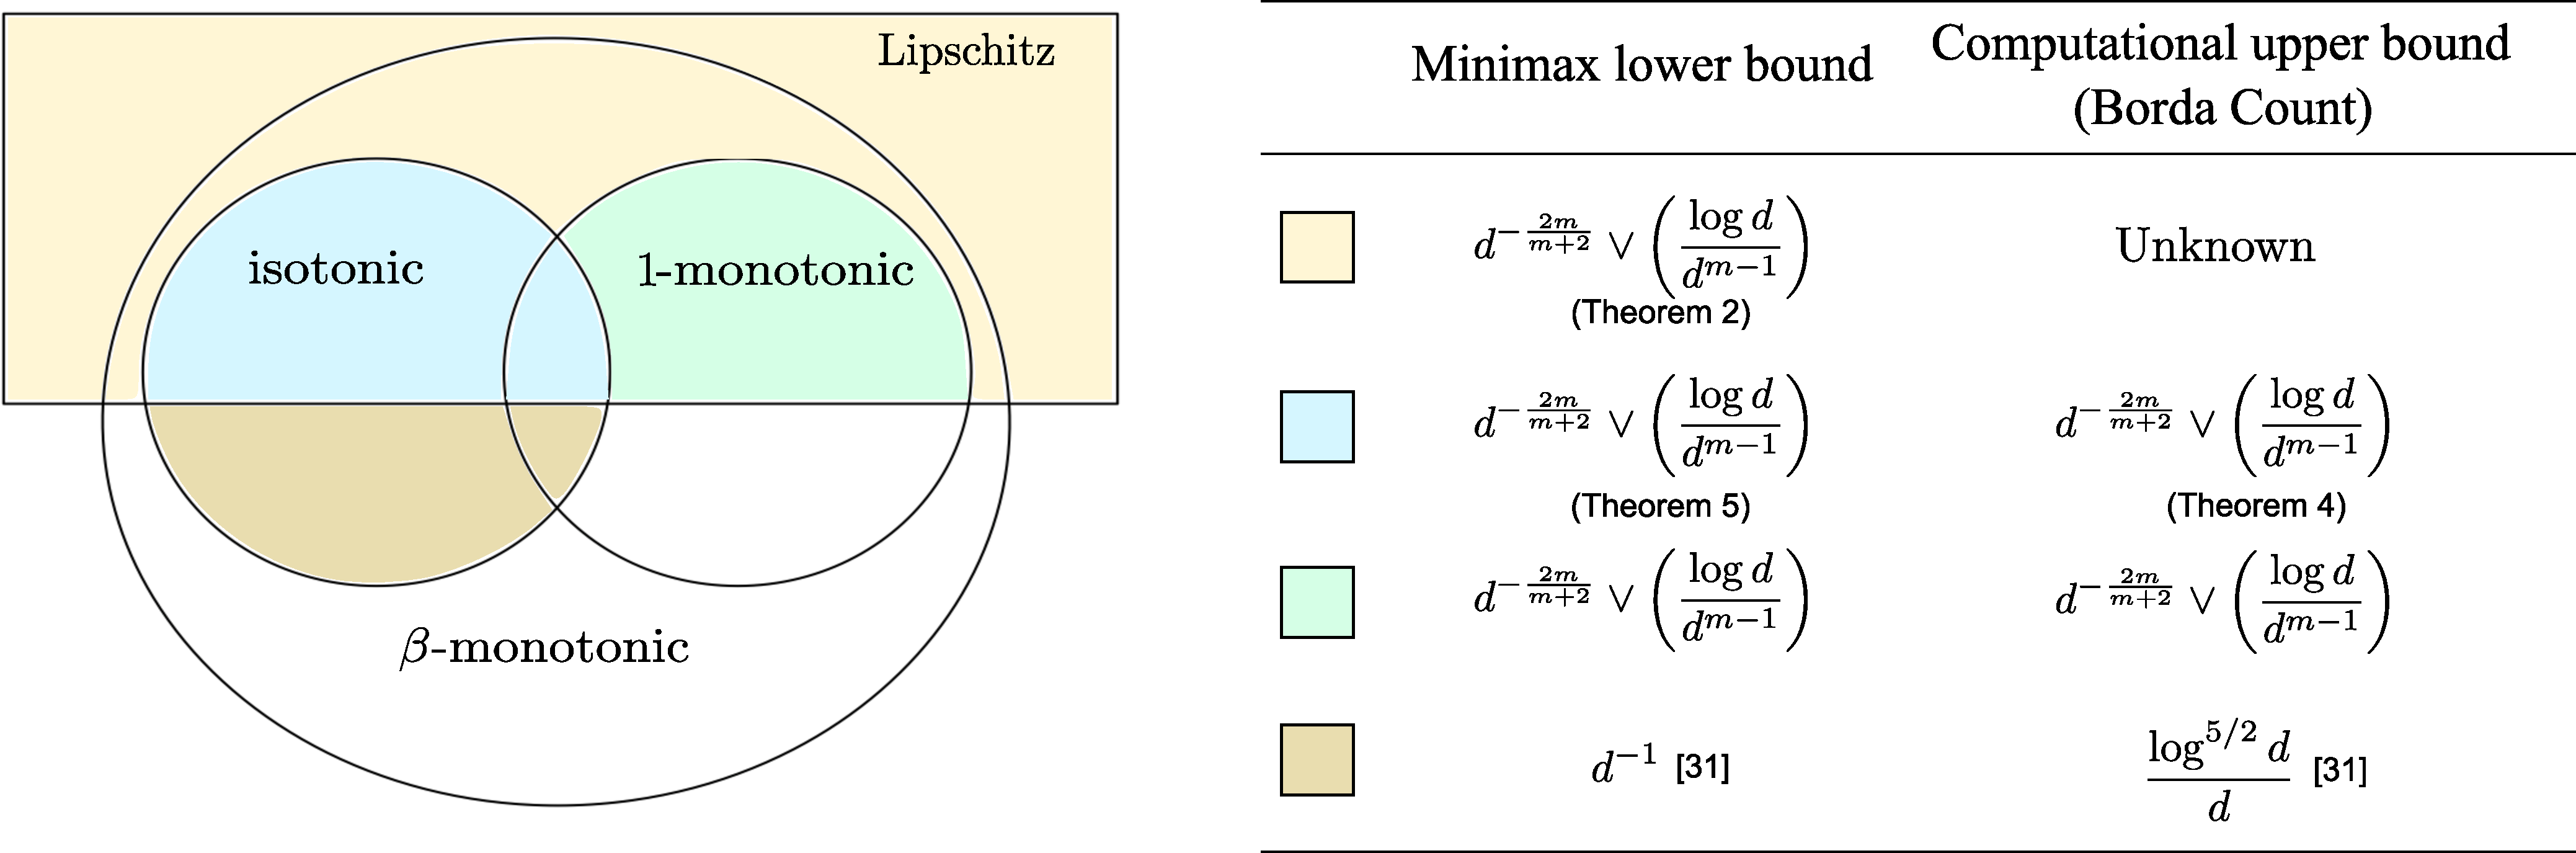
\includegraphics[width = 0.85\textwidth]{figure/Venn.pdf}
    \caption{\color{blue}Comparison of statistical lower bound and computational upper bound of Borda count algorithm.  The right table summarizes the statistical and computational rates corresponding to each colored region in the Venn diagram.}
    \label{fig:venn}
\end{figure}
}
\end{quote}

    
\item \textit{The question about the adaptivity of the algorithm.} 
    
\textbf{Response:} This is an important yet challenging question. We interpret the question as model selection; we address the issue from two perspectives. 

{\bf -- In practice}, we recommend to search $(k,\ell)$ via cross-validation in the algorithm. We have added the following subsection in Section 4: 

\begin{quote}
``\color{blue} ... {\bf Hyperparameter tuning.} Our algorithm has two tuning parameters $(k,\ell)$. The theoretically optimal choices of $(k,\ell)$ are given in Theorems~\ref{thm:LSE} and~\ref{thm:BC}. In practice, since model configuration is unknown, we search $(k,\ell)$ via cross-validation. 
Based on our theorems, a polynomial of degree $\ell^*=(m-2)(m+1)/2$ is sufficient for accurate recovery of order-$m$ tensors, whereas higher degree brings no further benefit. The practical impacts of hyperparameter tuning are investigated in Section 6. 
\end{quote}

In Section 6:
\begin{quote}
\color{blue}``...The first experiment examines the impact of the block number $k$ and degree of polynomial $\ell$ for the approximation....Figure 4 demonstrates the trade-off in accuracy determined by the number of groups for each polynomial degree...We find that degree-2 polynomial approximation gives the smallest MSE among considered polynomial approximations for models 1-7. By Remark~\ref{rm2}, plugging $(\alpha,m)=(\infty,3)$ in~\eqref{eq:choice} gives the theoretical choice $(k^*,\ell^*)=(d^{7/3},2)$. The results are consistent with our simulation.''
\end{quote}

{\bf -- In theory}, the development of tuning-free, adaptive algorithms is important. This general topic applies to all nonparametric problems, not only to our problem per se. We have added the following discussion in Section~\ref{sec:discussion}:

\begin{quote}
``...{\color{blue} Another limitation of our algorithm is the requirement of hyperparameter tuning. There is a vast literature on nonparametric estimation that focuses on adaptivity. For example, spatially adaptive methods have been developed in the contexts of wavelets~\citep{donoho1994ideal}, splines~\citep{mammen1997locally}, and trend filtering~\citep{tibshirani2014adaptive}; tuning-free algorithms have been proposed for several shape-constrained functions~\citep{chatterjee2019adaptive,feng2022nonparametric,bellec2018sharp}; see~\citep{cai2012minimax} for a review. Our work is orthogonal to these advances, and in principle we can combine these tools in our tensor estimation.} In this paper, we choose standard polynomial algorithm because of its simplicity. The parsimony leads to an easier analysis on the critical smoothness level $ (m-2)(m+1)/2$. Exploiting various nonparametric techniques for tensor models warrants future research.''
\end{quote}


\end{enumerate}

\newpage

\begin{center}
    \textbf{Point-by-point Response to Reviewer 1}
\end{center}

\emph{This manuscript deals with the interesting problem of estimating an order-$m$ $d$-dimensional tensor $\Theta$ which is $\alpha$-Holder smooth up to an unknown permutation $\pi$--for simplicity it is assumed that the permutation is the same along all modes. The main contribution is two-fold.}

\emph{First, the author introduce an (exp-time) estimator by minimizing the least-square criterion over all possible partitions of the $d$ points in $k$ block and then estimating the tensor $\Theta$ as a piece-wise polynomial degree-$\ell$ on these blocks. If one suitably tunes $k$ and $\ell$, the resulting estimator is shown to achieve the minimax estimation rate.}

\emph{Second, the authors introduce a simple efficient estimator under the additional $\beta$-monotonicity assumption. This assumption allows to almost exactly recover the permutation of the points by simply considering the Borda count of each point. Then, combining this estimated permutation with a piece-wise polynomial estimator allows the authors to recover the desired convergence rate.}

\emph{The paper is mostly well written. Numerical comparisons illustrate the results. Up to my knowledge, the minimax rate for smooth tensors (up to a permutation) is new. In comparison to the abundant literature for matrix or tensor estimations, the main novel idea is that of using a piece-wise polynomial estimator instead of a piecewise constant vector, which allows the authors to considering $\alpha$-smooth tensors with $\alpha > 1$.}

We greatly appreciate your valuable comments and suggestions. We have carefully addressed all the questions. Note that general comments raised by both reviewers were addressed upfront in {\bf pages 1-7 of this response letter, Response to Major Comments Summarized by Editor}. We will make explicit reference to earlier section when needed. 


\begin{enumerate}[wide, labelwidth=!, labelindent=0pt]
    \item \textit{I find the comparison of the results in Table 1 somewhat misleading. For instance, the row ``Polynomial algorithm" may suggest that there exists a Polynomial algorithm for general $\alpha$-smooth tensors, whereas a polynomial-time estimator is only exhibited under the very restrictive $\beta$-monotonicity assumption. In the row ``error rate" and columns ``$\alpha$-smoothness" the authors only state the rate for $\alpha=\infty$, whereas the rates for previous works are provided under much weaker regularity assumptions.}
    
    {\bf Response:} We have updated the table for fair comparison. 
    
    
 \begin{table*}[h]
    \centering
    \resizebox{\textwidth}{!}{%
    \begin{tabular}{c|@{\hskip4pt}c@{\hskip5pt}c@{\hskip4pt}c@{\hskip5pt}c@{\hskip4pt}c@{\hskip5pt}c@{\hskip4pt}c@{\hskip5pt}c@{\hskip5pt}c}
    & \citet{pananjady2022isotonic}&  \citet{balasubramanian2021nonparametric}&  \citet{li2019nearest}&\textbf{Ours} (MLE) & \textbf{Ours} (Borda count)\\
    \hline
       Model structure& monotonic & Lipschitz & Lipschitz &   \color{blue} $\alpha$-smooth  &  \color{blue} $\alpha$-smooth \& monotonic\\
        \color{blue}     Fixed grid design &  \color{blue}  $\surd$ &  \color{blue} $\times$ &  \color{blue}  $\times$ &   \color{blue} $\times$& \color{blue}  $\surd$\\
     Error rate for order-$m$ tensor & \multirow{2}{*}{$d^{-1}$} & $d^{-{2m\over m+2}}$ &   $d^{-\lfloor m/3\rfloor }$ &  \color{blue} $d^{-{2m\alpha\over m+2\alpha}}\vee d^{-(m-1)}$ & $ \color{blue}  d^{-{2m\alpha\over m+2\alpha}}\vee d^{-(m-1)}$ \\
       (e.g., when $(m,\alpha)=(3,1)$) & & ($d^{-6/5}$) & $(d^{-1})$ & $(d^{-6/5})$ & $(d^{-6/5})$\\
          Minimax optimality& $\surd$  & $\times$ & $\times$ & $\surd$ & \color{blue}$-*$ \\
     Polynomial algorithm& $\surd$ &$\times$ & $\surd$ & $\times$& \color{blue}$\surd$ 
    \end{tabular}
    }
    \caption{Comparison of our results with previous work. For simplicity, we omit the log term in the rate. \color{blue}$^{*}$Optimality is achieved under extra Lipchitz monotonicity conditions. }\label{tab:comp}
\end{table*}

    
    We also add new theorem to show the \emph{non-existence} of polynomial-time algorithm achieving the minimax rate without further assumption (see \textbf{Point 1 in Response to Major comments Summarized by Editor} for details). We present two estimation algorithms in the revised table: the maximum-likelihood estimation (MLE) and the Borda count estimation. The MLE uses no extra assumption and improves the previously conjectured optimal rate in the earlier work~\citep{balasubramanian2021nonparametric}. The Borda count algorithm achieves efficiency under an extra Lipschitz condition (see \textbf{Points 1-2 in Response to Major comments Summarized by Editor} for details). 
    
        
    \item \textit{I have concerns with the proof of the minimax lower bound (Theorem 2). More precisely, I do not understand how one deduces (31) from (29), (30), and Lemma 4 in Page 44. Informally, in (29), the authors reduce their problem to that of estimating a block-constant tensors (up to a permutation) of ($d/2$) points, while knowing exactly the position of the $d/2$ remaining points. As as consequence, this does not boil down to the setting of Lemma 4, as the statistician also observes all the interactions between the $d/2$ points with known position and the $d/2$ points with unknown position. This additional information could make the problem significantly easier than what is suggested by Lemma 4. Could the authors elaborate on that?}
    
     \textbf{Response:} Thank you for pointing out the gap omitted in the proof. We have added the following lines in the proof to address your concern.
     \begin{quote}
``The proof of Lemma~\ref{lem:permutation} is constructive and deferred to Section~\ref{sec:tech}. {\color{blue}The core tensor $\tS$ in Lemma~\ref{lem:permutation} has a special pattern of zero's that will be used in the proof of Theorem~\ref{thm:minimax}; see the Section~\ref{sec:tech} for details....}

``...From this observation, we define a sub-domain $I\subset [d]$ such that
\begin{align}\label{eq:2}
    I = \left(\bigcup_{a=1}^k\left[\frac{d(a-3/4)}{k},\frac{d(a-1/4)}{k}\right]\right)\bigcap [d].
\end{align}
We have that $|I|=d/2$ by definition. Let $\Theta(\tS)\in\mathbb{R}^{d\times \cdots \times d}$ denote the tensor induced by $f$ in~\eqref{eq:constructf}. We use subscript $I$ to denote objects when restricted in the indices set $I$. For example, $\Theta_I(\tS)\in\mathbb{R}^{d/2 \times \cdots \times d/2}$ denotes the sub-tensor with indices in $I$, and $\normSize{}{\cdot}$ denotes the sum of squares over indices in $I$. Based on~\eqref{eq:1} and~\eqref{eq:2}, $\Theta_I(\tS)$ has block structure with the core tensor $\tS$. 

{\color{blue}We use $\Pi(d/2,d/2)$ to denote the set of all permutations on $I$ while fixing indices on $[d]\setminus I$; that is, $\Pi(d/2,d/2)=\{\pi\colon I\to I\}\cong \{\pi\in\Pi(d,d)\colon \pi(i) = i \text{ for } i\in[d]\setminus I\})$. Then, we have
\begin{align}
&\inf_{(\hat \Theta,\hat \pi)}\sup_{\pi\in \Pi(d,d)}\mathbb{P}\left({1\over d^m}\FnormSize{}{\hat \Theta\circ \hat \pi-\Theta(\tS)\circ \pi}^2\geq \varepsilon^2\right)\notag \\
\stackrel{(*)}{=}&\ \inf_{\hat \Theta}\sup_{\pi\in \Pi(d,d)}\mathbb{P}\left({1\over d^m}\FnormSize{}{\hat \Theta-\Theta(\tS)\circ \pi}^2\geq \varepsilon^2\right)\notag \\
\geq &\ \inf_{\hat \Theta}\sup_{\pi\in \Pi(d,d)}\mathbb{P}\left({1\over d^m}\normSize{}{\hat \Theta-\Theta(\tS)\circ \pi}^2\geq \varepsilon^2\right)\notag \\
\stackrel{(**)}{\geq}& \ \inf_{\hat  \Theta}\sup_{\pi \in\Pi(d/2,d/2)}\mathbb{P}\left({1\over (d/2)^m}\FnormSize{}{\hat \Theta_{I}-\Theta_{I}(\tS)\circ \pi}^2\geq 2^m\varepsilon^2\right)\notag \\
= & \ \inf_{\hat  \Theta}\sup_{z\in \Pi(d/2,k)}\mathbb{P}\left({1\over (d/2)^m}\FnormSize{}{\hat \Theta_I-\tS\circ z}^2\geq 2^m\varepsilon^2\right),
\end{align}
where $(*)$ absorbs the estimate $\hat \pi$ into the estimate $\hat \Theta$, and $(**)$ uses the constructed function \eqref{eq:constructf} and the permutation collections $\Pi(d/2,d/2)$. Based on the construction of $\tS$ in Lemma~\ref{lem:permutation}, the cross terms in $(\tS\circ z) (I, I^c, \ldots)$ are zero. Therefore, we reduce the problem of estimating $\pi \colon [d]\to[d]$ to estimating $z: I\to[k]$ in the sub-tensor. Applying Lemma~\ref{lem:permutation} to\eqref{eq:lower} by using $d/2$ in the place of $d$ and $k=d^{\delta} $ for a constant $\delta>0$ yields the desired conclusion. 

Note that we observe all interactions between the $d/2$ points with known position and $d/2$ points with unknown positions. This addition information occurs only a constant $2^m$ factor in the final bound, due to zero patterns in the core tensor $\tS$ in Lemma~\ref{lem:permutation}. Since order of tensor $m$ is fixed, this improvement does not affect the final rate.
     }
     \end{quote}
     

     
     \item \textit{ First, I am wondering whether the minimax rate should not be faster under this assumption as one could perhaps leverage on this assumption to improve the non-parametric rate. }
     
     \textbf{Response:} 
Inspired by your comments, we have added a new Theorem~\ref{thm:mminimax} to provide the minimax rate under monotonicity. It turns out the monotonicity does not improve the rate under Lipschitz condition (equivalently, $\alpha=\beta=1$ in our setting). The high-level idea is based on the \citet{mark2002} and the referred proof in~\citet{kiefer1982}:
\begin{quote}
``(page 364 of  \citet{mark2002})...this extra order constraint (monotone) does not improve optimal rates of convergence..., and thus $d^{-2\alpha/(2\alpha+1)}$ is still the optimal rate of convergence for the minimax risk (for 1-d function estimation)...''
\end{quote}

Please see detailed response in \textbf{Point 2, Response to Major Comments summarized by Editor (pages 1-7 of this letter)}.  
%We have added the proof of the minimax rate for $\tF(1,L)\cap\tM(1)$. %We conjecture that similar results hold true when the nonparametric error dominates the rate (e.g., $\alpha<c(\alpha,\beta,m)$ in~\eqref{eq:rateBC}). For general $(\alpha,\beta)$, the optimality is unknown; we discuss the proof challenges in Appendix~\ref{subsec:generala}.  
          
     \item \textit{Second, contrary to what is stated in the manuscript, this assumption is not weaker than an isotonic condition. Indeed, isotonic condition prescribe that the difference $g(i) - g(j)$ is non-negative, but not that this different is at least of the order $(i - j)^\beta$. }
        
      \textbf{Response: }
      The isotonicity belongs to our monotonic model by setting $\beta=\infty$ in $|i-j|^\beta$ based on Definition 2 in the paper\footnote{Our paper uses the notion of $|i-j|^{1/\beta}$, so $\beta=0$ in our notation.}. To see this, set $|i-j|=1$ and $\beta=\infty$. Then $g(i)-g(j)\geq (|i-j|/d)^\beta\to 0$ as $d\to\infty$, reducing to the free-of-order constraint. This is what we meant by the broadness of our framework. 
      
      Furthermore, our $\beta$-monotonicity model considers the \emph{marginal} monotonicity, while the classical isotonicity model concerns the \emph{joint} monotonicity. The former is a weaker assumption. 
      
      
     We have added the following comment in Section 5.3
\begin{quote}
{\color{blue}


``One may also consider other assumptions such as isotonic functions~\citep{pananjady2022isotonic}. 
Define an isotonic function class $\tM$ 
\begin{align}\label{eq:iso}
    \tM = \{f\colon[0,1]^m\rightarrow\mathbb{R}\ \big| \ f(x_1,\ldots,x_m)\leq f(x_1',\ldots,x_m')\text{ when } x_i\leq x_i' \text{ for } i\in[m]\}.
\end{align}
The isotonic functions~\eqref{eq:iso} concerns the \emph{joint} monotonicity, where as our monotonicity~\eqref{eq:bdefn} concerns the \emph{marginal} monotonicity. The later is a weaker assumption. The latter is a weaker assumption. The isotonic functions belong to $\tM(0)$ based on our Definition~\ref{eq:bdefn}. Therefore, all our upper bounds apply to isotonicity functions, although such extension is not necessarily sharp. The extension of sharp bounds in Theorems~\ref{thm:BC}-5 to isotonic functions can be found in Appendix~\ref{sec:genminimax}.''
}
\end{quote}

We also added Figure~\ref{fig:venn} in the main paper to illustrate the relationship between isotonicity and monotonicity. The $\infty$-monotonicity includes isotonicity, while the $1$-monotonicity overlaps with isotonicity. Please see our response to {\bf Point 2, Response to Major Comments summarized by Editor (pages 1-7 of this letter)}. 

\begin{figure}[h]
    \centering
    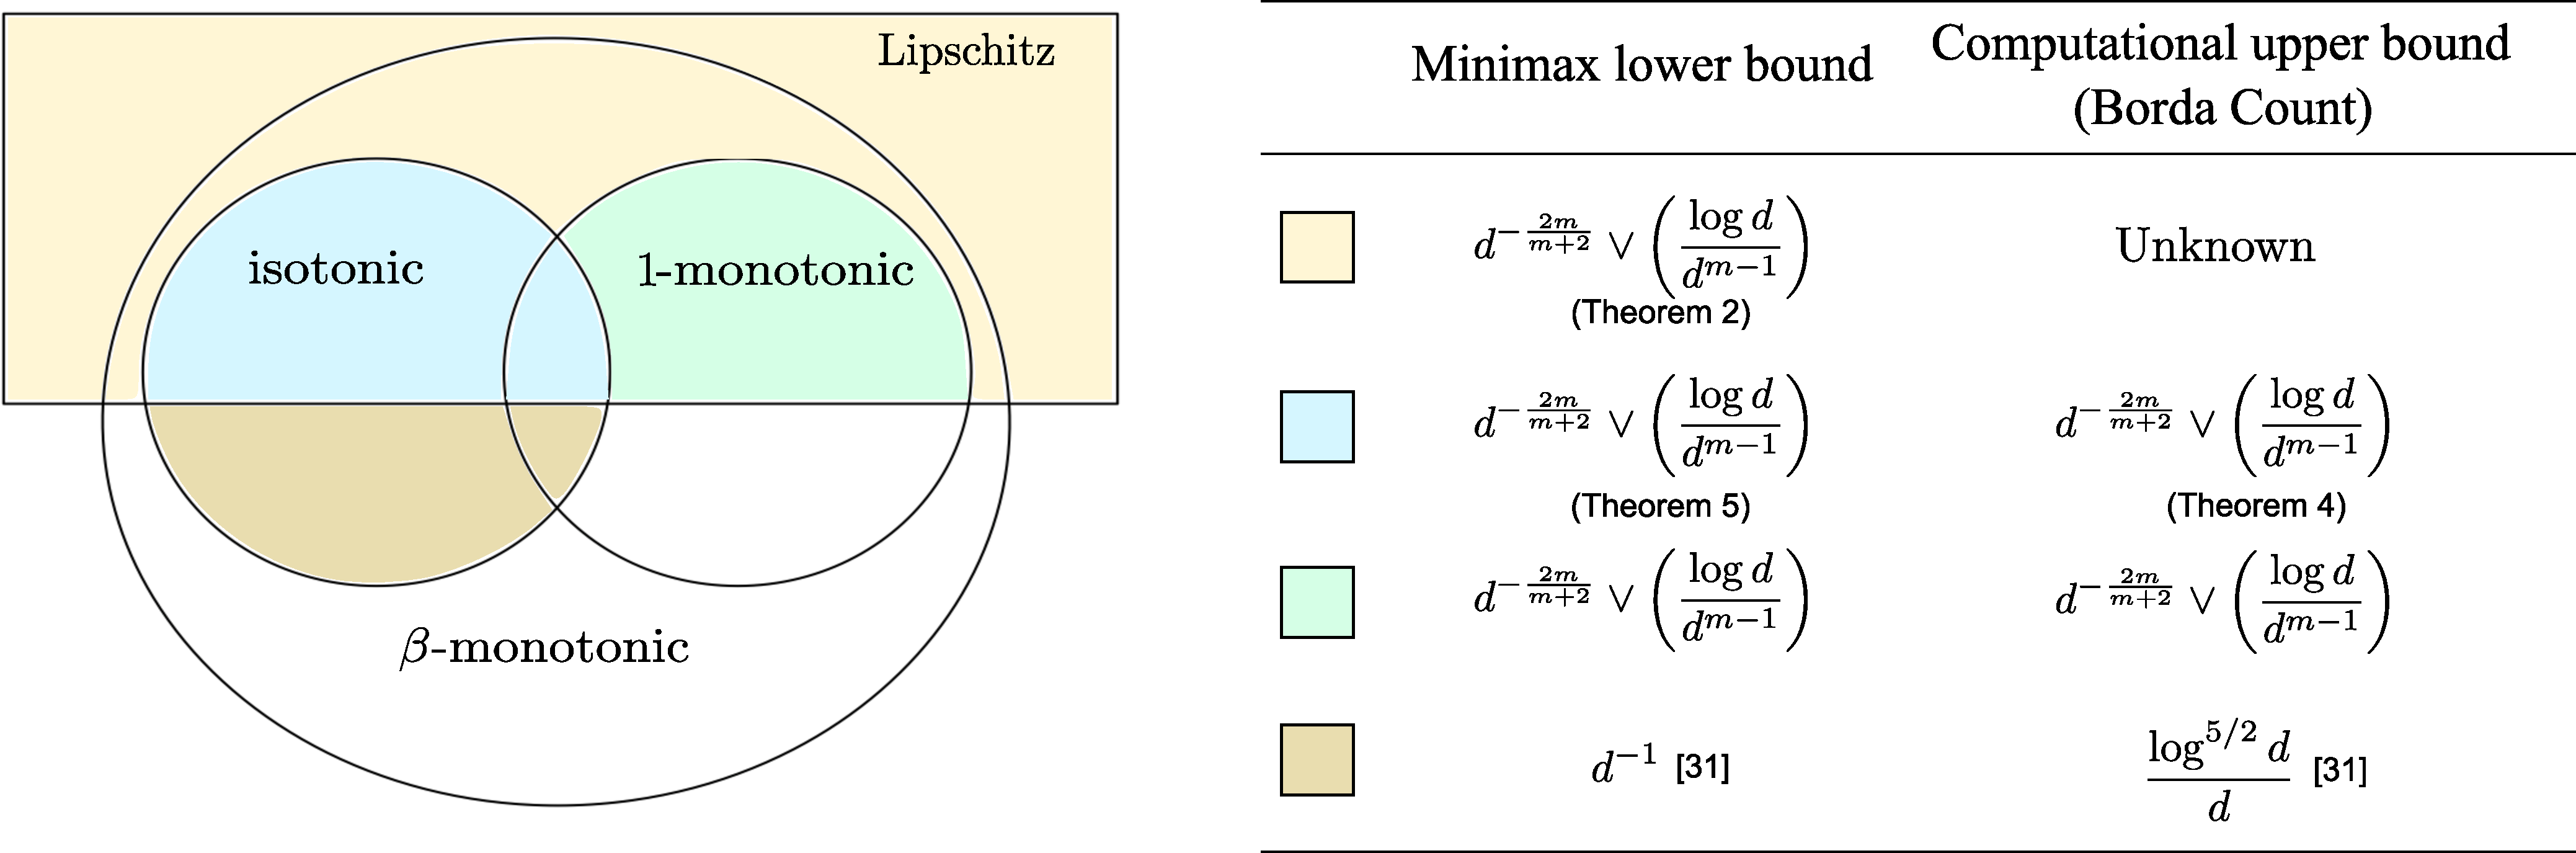
\includegraphics[width = 0.85\textwidth]{figure/Venn.pdf}
    \caption{\color{blue}Comparison of statistical lower bound and computational upper bound of Borda count algorithm.  The right table summarizes the statistical and computational rates corresponding to each colored region in the Venn diagram.}
    \label{fig:venn}
\end{figure}


     
     \item \textit{Are the authors able to address the isotonic case with their procedure?}
     
      \textbf{Response: } Based on our response to \#4, the isotonicity is a special case of our monotonicity. Therefore, all our upper bound results equally apply to isotonic functions. The lower bound results, however, need extra work. We summarize our new results in our response to {\bf Point 2, Response to Major Comments summarized by Editor (pages 1-7 of this letter)}. 
       

     
     
     
     
     
     
     \item \textit{Minor comments: }
     \begin{enumerate}
     \item \textit{Page 9, Line 46 ``Frobunis"}
        
         
    \item \textit{There is a typo in the subscript of (28)} 
    \item \textit{Lemma 5 (prosy)}
\end{enumerate}
\textbf{Response:} Thank you for the comments.  We have corrected the typos. 
\end{enumerate}



\newpage
\begin{center}
    \textbf{Point-by-point Response to Reviewer 2}
\end{center}

 \emph{The paper considers a permuted smooth tensor model (which is essentially an $m$-dimensional regression problem with unknown correspondences) in the fixed design setup and establishes minimax lower bounds and an estimator that achieves the lower bounds when the true regression function is $\alpha$-Holder. The main observation is that while prior works considered estimators which were based on piecewise constant approximations, the paper uses piecewise polynomial approximations (with the order of the polynomial picked accordingly). This enables the paper to obtain rates that are minimax optimal. A main issue (as with all prior works) is that the algorithm involves combinatorial search and hence is computationally hard.}
 
  \emph{The paper then propose an algorithm, based on the so-called Borda counts that provides a linear time algorithm (i.e., linear in dm, the number of entries). However, this requires the more stringent assumption that the true regression function is monotonic. Given this assumption, indeed the algorithm seems a natural algorithm to consider.}
  
 \emph{I have went over the proofs and they seem to be ok to my knowledge. The paper indeed makes a contribution to this growing literature. Hence, I recommend a major revision that would address the following concerns.}

We greatly appreciate your valuable comments and suggestions. We have carefully addressed all the questions. Note that general comments raised by both reviewers were addressed upfront in {\bf pages 1-7 of this response letter, Response to Major Comments Summarized by Editor}. We will make explicit reference to earlier section when needed. 

\begin{enumerate}[wide, labelwidth=!, labelindent=0pt]
    \item \textit{The paper claims the proposed Borda count algorithm is both statistically and computationally efficient. However, the algorithm requires the more stringent assumption of monotonicity. Hence, I personally think this claim is a bit misleading. In fact, it is not clear what is the minimax lower bound for when the truth lies in $\tF(\alpha, L) \cap \tM(\beta)$.  }
    
    
    \textbf{Response:} 
    Inspired by your comments, we have added a new theorem 5 to show the minimax lower bound for $\tF(1,L)\cap \tM(1)$. The rate turns out to agree with Borda count algorithm. We conjecture that similar results hold true when the nonparametric error dominates the rate (e.g., $\alpha<c(\alpha,\beta,m)$ in~\eqref{eq:rateBC}). For general $(\alpha,\beta)$, the optimality is unknown; we discuss the proof challenges in Appendix~\ref{subsec:generala}.  



   
Please see our detailed revision in \textbf{Point 2, Response to Major Comments summarized by Editor (pages 1-7 of this letter)}. Throughout the paper, 
the new conclusion now reads ``...Borda count algorithm achieves optimal rate {\color{blue}under an extra Lipchitz monotonic condition''}.      

     \item \textit{Furthermore, can the authors provide some intuition about this class $\tF(\alpha, L) \cap \tM(\beta)$ ? }
     
     \textbf{Response: } We have added the following descriptions in Section 5:
\begin{quote}
\color{blue}
``...We refer to $\tF(\alpha,L)\cap \tM(\beta)$ as the monotonic-plus-smooth function class. This class was initially proposed in previous literature of graphons. The work~\citep{chan2014consistent} proposes the Lipschitz monotonic function to facilitate the analysis of sorting-merging algorithm for matrix estimation; their setting is a special case of our Definition 2 with $(\alpha,\beta,m)=(1,1,2)$. Inspired by earlier work, we consider the similar monotonic-plus-smooth function class $\tF(\alpha,L)\cap \tM(\beta)$ under general configuration $\{(\alpha,\beta,m): \alpha>0,\ 0<\beta\min(\alpha,1)\leq 1, \ m\geq 2\}$. ...
\end{quote}

     We added Figure~\ref{fig:venn} in the main paper for the intuition about function classes. Figure~\ref{fig:venn} summarizes the relationship among various function classes and corresponding statistical and computational limits. The function class of $\tF(\alpha,L)$ concerns the smoothness, while $\beta$-monotonicity concerns marginal monotonicity. Please see our response to {\bf Point 2, Response to Major Comments summarized by Editor (pages 1-7 of this letter)}. 
     
     
\setcounter{figure}{2}
\begin{figure}[h]
    \centering
    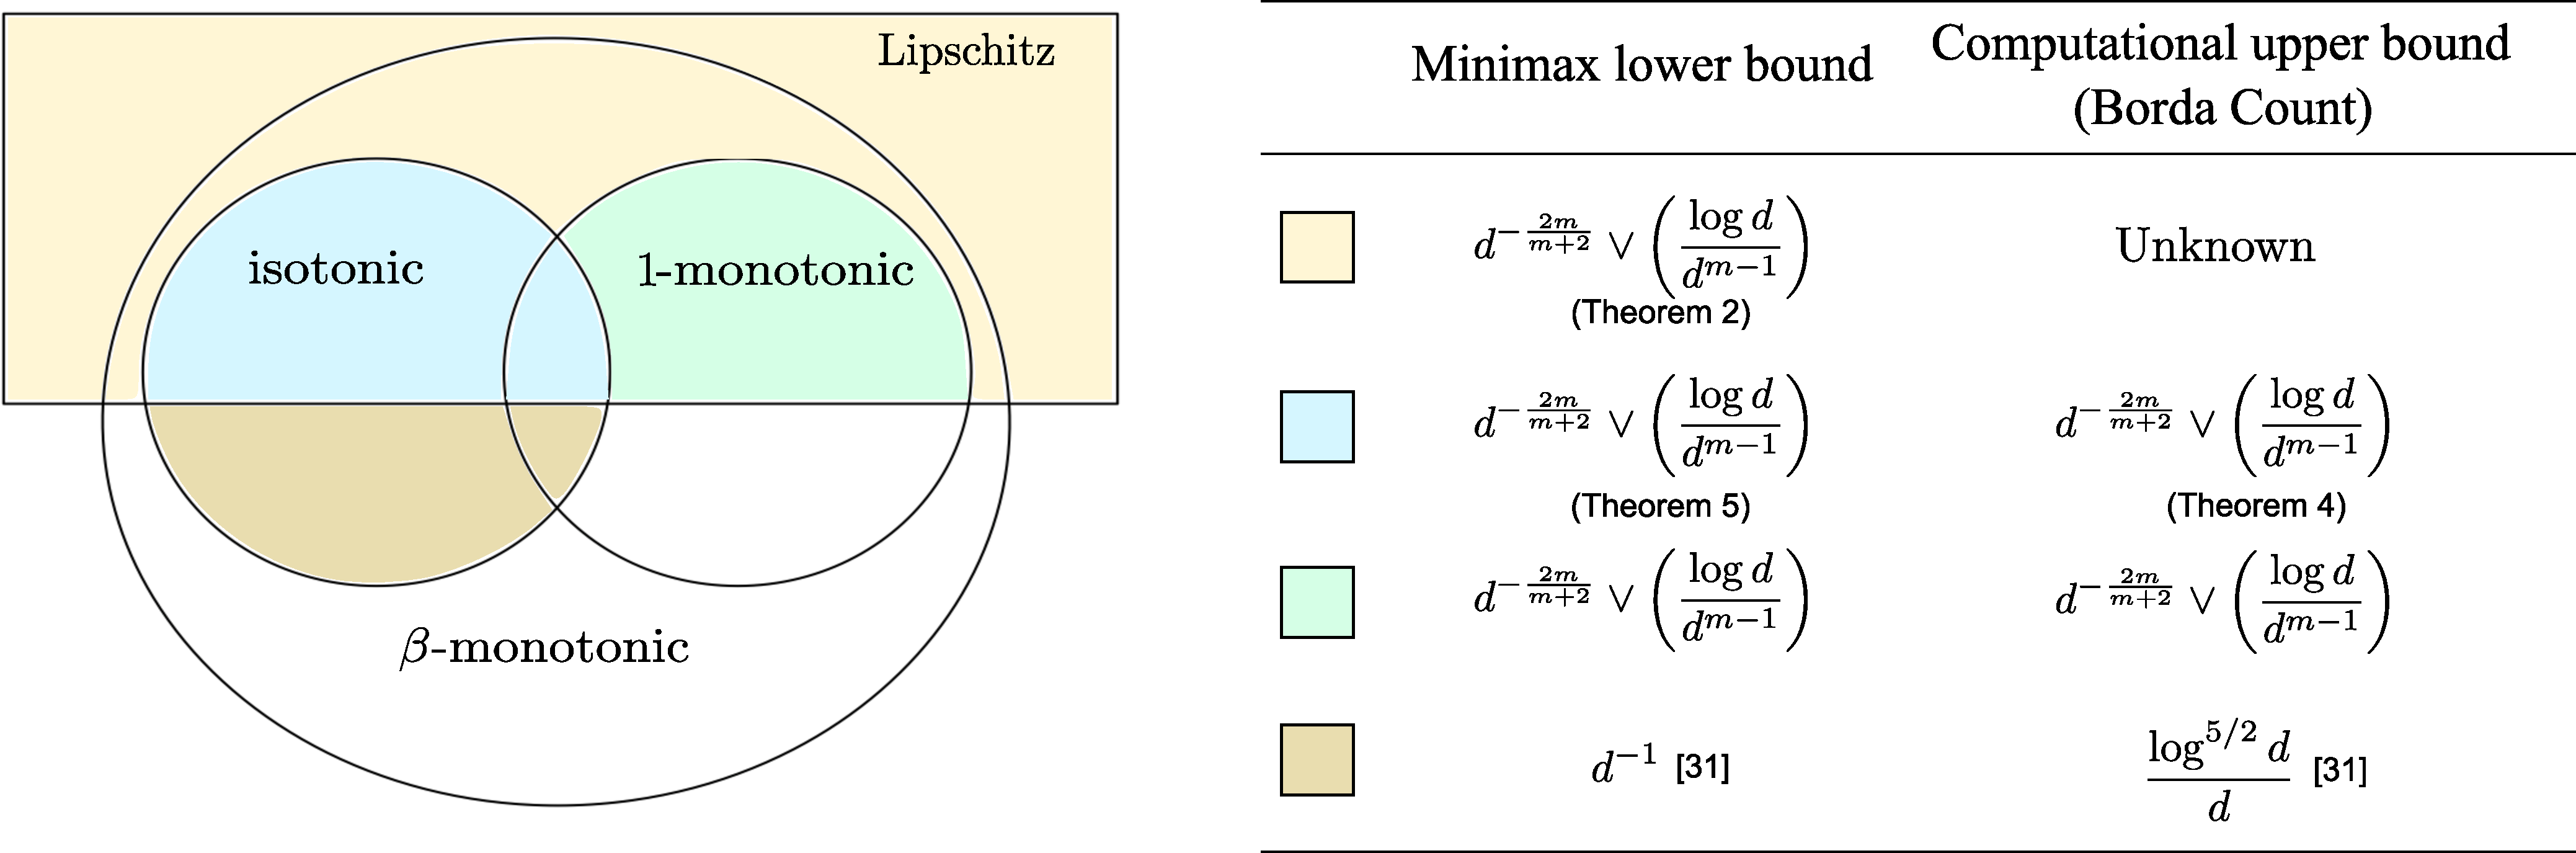
\includegraphics[width = \textwidth]{figure/Venn.pdf}
    \caption{\color{blue}Comparison of statistical lower bound and computational upper bound of Borda count algorithm.  The right table summarizes the statistical and computational rates corresponding to each colored region in the Venn diagram.}
\end{figure}
    
    
     \item \textit{Do the examples in Model 1 to 5 belong to this class ? }

\textbf{Response: }   Yes, all examples in Models 1 to 5 belong to this class. We added the last two columns in Table~\ref{tb:md} to present the corresponding model configuration $(\alpha,\beta)$ for models 1-5. 
    
    \begin{table}[H]
    \centering
    \begin{tabular}{c|c|c|c|c|c}
        Model ID  &  $f(x,y,z)$ & CP rank & Tucker rank &  ${\color{blue}\geq(\alpha,\beta)}$ & Isotonic \\\hline
        1 &    $xyz$ & 1 & $(1,1,1)$ & ${\color{blue}(\infty, 1)}$ &$\surd$ \\
        2 &    $(x+y+z)/3$ & 3 & $(2,2,2)$ & ${\color{blue}(\infty,1)}$&$\surd$\\
        3 & $(1+\exp(-(3x^2+3y^2+3z^2))^{-1}$ &9& $(4,4,4)$ & ${\color{blue}(\infty,1/2)}$ &$\surd$\\
        4 & $\log(1+\max(x,y,z))$ &$\geq 100$& $\geq (50,50,50)$ &${\color{blue}(1,1)}$&$\surd$\\
        5 &  $\exp\left(-\max(x,y,z)-\sqrt{x}-\sqrt{y}-\sqrt{z}\right)$ &$\geq 100$& $\geq (50,50,50$) & ${\color{blue}(1/2,1)}$ &$\surd$
    \end{tabular}
    \caption{\color{blue}Smooth functions in simulation. ...}
\end{table}
    
    \item \textit{Adaptivity: Both in Theorems 1 and 3, the result requires knowledge of $\alpha$. In theorem 3, in addition knowledge about $\beta$ is required. Could the authors extend their results so that they are adaptive to the choices of $\alpha$ and $\beta$?}
    
    \textbf{Response:} 
  This is a great question. We interpret the adaptivity as a model selection problem. Please see \textbf{Point 3, Response to Major Comments summarized by Editor (pages 1-7 of this letter)}.
        
    \item \textit{Furthermore, from the experiments, it is not clear how the observed empirical choices of $({\ell}^*,k^*)$ are related to the theoretical choices. The authors mention that these observations are consistent with our theoretical results that the optimal number of blocks and polynomial degree are $(k^*,\ell^*) = (\tO(d^{3/7}),2)$. However this is not clear at all. Can the authors calculate the theoretical choices for models 1 to 5 and show it agrees with the simulation ?}
    
    \textbf{Response:} 
    Thank you for the comments. In the Remark~\ref{rm2} of the main paper, we show that, 
    
    \begin{quote}
    \color{blue}...when the generative function is infinitely smooth ($\alpha =\infty$) with Lipschitz monotonic score $(\beta=1)$, ... (the optimal rate is achieved) under the choice of degree and block number
\[
\ell^*= {(m-2)(m+1)/2}\quad \text{ and } \quad k^* \asymp d^{m\over m +2(\ell^*+1)}.
\]
\end{quote}

In the simulation models, we plug in $(\alpha, m)=(\infty, 3)$ to obtain $(k^*,\ell^*) = (d^{7/3},2)$. Therefore, the theoretical choice agrees with the simulation. 

We added the following paragraph in the main paper for a clear explanation:       
    \begin{quote}
In addition, we find that degree-2 polynomial approximation gives the smallest MSE {\color{blue}among considered polynomial approximations for models 1-7. By Remark~\ref{rm2}, plugging $(\alpha,m)=(\infty,3)$ in~\eqref{eq:choice} gives the theoretical choice $(k^*,\ell^*)=(d^{7/3},2)$ . The results are consistent with our simulation. }
    \end{quote} 
    
    
   
    
    \item \textit{Also, to my knowledge, the papers [1] and [18] seem to consider random design setup. It is not clear if Table 1 is a fair comparison in this sense. This distinction should perhaps be distinguished right in the introduction rather than in the conclusion section at the end. Furthermore, how is the fixed-design assumption verified for the Chicago crime dataset experiment?}
    
    \textbf{Response:}
       We revised the Table 1 for fair comparison. The newly added rows are highlighted in blue. 
   \begin{quote}
   \begin{table*}[h]
    \centering
    \resizebox{\textwidth}{!}{%
    \begin{tabular}{c|@{\hskip4pt}c@{\hskip5pt}c@{\hskip4pt}c@{\hskip5pt}c@{\hskip4pt}c@{\hskip5pt}c@{\hskip4pt}c@{\hskip5pt}c@{\hskip5pt}c}
    & \citet{pananjady2022isotonic}&  \citet{balasubramanian2021nonparametric}&  \citet{li2019nearest}&\textbf{Ours} (MLE) & \textbf{Ours} (Borda count)\\
    \hline
       Model structure& monotonic & Lipschitz & Lipschitz &  $\alpha$-smooth  & $\alpha$-smooth \& monotonic\\
               \color{blue} Fixed grid design &  \color{blue} $\surd$ & \color{blue} $\times$ &  \color{blue} $\times$ &  \color{blue} $\times$&  \color{blue} $\surd$\\
       \vdots &    \vdots&\vdots&\vdots&\vdots&\vdots\\
     Polynomial algorithm& $\surd$ &$\times$ & $\surd$ & $\times$& $\surd$ 
    \end{tabular}
    }
    \caption{\color{blue}Comparison of our results with previous work...}
\end{table*}
     \end{quote}
     
     \vspace{-1cm}
   We have also added the following clarification in Section~1.2:    
   \begin{quote}
   \color{blue}``...Unlike typical simple hypergraphons where the design points are random, our generative model uses deterministic design points. These two choices lead to different analysis similar as random- vs.\ fixed-designs in nonparametric regression~\citep{wasserman2006all,tsybakov2009introduction}. The comparison of two approaches will be discussed in Sections 2~and~4.''
   \end{quote}
   
In Section 2, we have added:
\begin{quote}
{\color{blue}``...Our model~\eqref{eq:rep} assume equally-spaced grid design $\{1/d,2/d,\ldots,d/d\}$ from the generative function $f$. One can also extend the model to allow non-equally-spaced designs. Specifically, suppose that the signal tensor is generated from $f$ based on 
\begin{align}\label{eq:randommodel}
\Theta(i_1,\ldots,i_m) = f(x_{i_1},\ldots,x_{i_m}), \quad \text{for all} \quad (i_1,\ldots,i_m)\in[d]^m. 
\end{align}
where the points $\{x_i\}_{i=1}^d$ can be modeled as either fixed latent variables or i.i.d.\ random variables from a probability distribution supported on $[0,1]$. We refer to~\eqref{eq:randommodel} as the relaxed smooth model; similar model has been developed in the literature of graphons and hypergraphons~\citep{chan2014consistent,gao2015rate,klopp2017oracle,balasubramanian2021nonparametric}. Our paper will focus on the grid design~\eqref{eq:rep}, but we will also discuss the extension to~\eqref{eq:randommodel} whenever possible as remarks of theorems.}      
\end{quote}

In Section 4, we added:
\begin{quote}
{\bf Remark~\ref{rmk:phase}} (Phase transition). {\color{blue} Our Theorem~\ref{thm:LSE} can be extended to relaxed smooth model~\eqref{eq:randommodel}. In the Appendix~\ref{sec:rdesign}, we show that the relaxed smooth model has the same convergence upper bound $\text{Rate}(d)$, with little modification of proofs.} 
\end{quote}

In the conclusion Section, we added:
\begin{quote}
 {\color{blue}We find that our theorems in Section~\ref{sec:lse} can be extended to random designs; the analysis is provided Appendix~\ref{sec:rdesign}. The extension of theorems in Section~\ref{sec:borda}, however, remain challenging for random designs. A full comparison between the two designs is an interesting question for future research.
 }
\end{quote}

We also add a new Appendix~\ref{sec:rdesign} to prove the extension of Theorem~\ref{thm:LSE} and Proposition~\ref{lem:approx} to random design models. 

Similar to other papers \citep{balasubramanian2021nonparametric,li2019nearest}, we do not present a statistical test for checking whether the fixed or random design assumption is true in real data application. In our Chicago crime data analysis, we use domain knowledge to validate output results. We believe that verifying nonparametric model assumptions (not restricted to our framework) in real data is generally challenging, and we leave it for future work. 
     
    
    \item \textit{Minor comments: Reference [23] and its citation in Lemma 6 needs to be fixed.}
  
   \textbf{Response:} Thank you for the comments. We have fixed the reference [23] and its citation.
    
\end{enumerate}

\newpage

\begin{center}
    \textbf{Point-by-point Response to Reviewer 3}
\end{center}


\emph{This paper proposes a permuted smooth tensor model, where the mean of the observation at $(i_1,i_2,\ldots,i_m)$ is equal to $f(i_1/d, i_2/d,\ldots,i_m/d)$, for a smooth $m$-variate function $f$, subject to an unknown permutation of indices. The authors studied the minimax estimation error when $f$ belongs to a Holder class and achieved this rate by a (computationally expensive) least-squares algorithm. The authors also proposed a Borda count algorithm, for the special case where $f$ is both smooth and monotone, and showed that it achieves the minimax rate in this case. The algorithm is applied to the Chicago crime count data and produces some interesting results, such as clustering of neighborhoods.}

\emph{The paper is very well-written. The methods and main contributions are stated clearly. There are also many interpretations of theory (e.g., why the order should have such a form, how it compared with the error orders in related problems). These interpretations help the readers understand the insights behind the theory, which I really like.}


We greatly appreciate your valuable comments and suggestions. We have carefully addressed all the questions. Note that general comments raised by both reviewers were addressed upfront in {\bf pages 1-7 of this response letter, Response to Major Comments Summarized by Editor}. We will make explicit reference to earlier section when needed. 


\begin{enumerate}[wide, labelwidth=!, labelindent=0pt]
    \item \textit{My main concern is that the problem has not yet been fully resolved. I was hoping to see a more complete answer. Without monotonicity, how to develop a polynomial-time algorithm? }
    
    
    
\textbf{Response: }
We added new results from two perspectives:

{\bf -- In theory,} we have improved our results inspired by your comments. We add a new section 5.1 with a new Theorem 3, which roughly says:

\begin{quote}
\color{blue}
``There exists \emph{no} polynomial-time algorithm that achieves the minimax statistical bound in the general setting, under the popular computational hardness conjecture on hypergraphic planted clique (HPC) detection and some technical conditions.''
\end{quote}
    Please see \textbf{Point 1, Response to Major Comments summarized by Editor (pages 1-7 in this letter)} for more details. Our new theory has suggested the need of extra assumptions for efficient polynomial-time algorithms. 
 

  {\bf -- In algorithm,} we added several new polynomial-time algorithms in the paper. In particular, the \textbf{\small LSE} in simulation is developed by us, and we treat it as a polynomial-time surrogate to MLE. This algorithm uses spectral method for initialization and constant blocks for approximation~\citep{han2022exact}. The comparison is provided in Section 6 and the new Figure R2 in this letter. Please see our responses to \# 5 and \#7 for details. 
 
    
    \item \textit{ Under this assumption, the unknown permutation is found by ordering the degrees of nodes. This prevents some common cases such as f being a quadratic function, e.g.,
    \begin{equation}\label{eq:example}
        f(x,y,z)=(x-0.5)^2 +yz.
    \end{equation}
    In this case, if we use Borda count to permute and group nodes in mode 1, the algorithm will mistakenly group together those top-ranked and bottom-ranked (in true ordering) nodes. I am wondering whether there exists an algorithm to deal with the general case without monotonicity. It is okay even if this algorithm doe not have the minimax rate. The current paper does not give any computable algorithm in the general case. This is the main weak-ness of the paper.}   

        \textbf{Response:} In fact, your quadratic function~\eqref{eq:example} falls precisely in our model class. The function is non-monotonic per se, but it is monotonic \emph{up to permutations.} Our Borda count algorithm works perfectly in your example~\eqref{eq:example}.
      
    We elaborate our response from three perspectives: \\  
    {\bf -- Your specific example (theory).} We demonstrate the success of our Borda count algorithm for smooth-plus-monotonic functions \emph{up to permutations.} This permutation needs not to be the same as the oracle permutation in the generative model. 
    
    We show that Borda count algorithm works perfectly on your example~\eqref{eq:example}. For simplicity, assume that $d$ is an even number. The signal tensor is represented by
    \begin{align}\label{eq:model6}
       \Theta(i,j,k) = \left(\frac{i}{d}-0.5\right)^2+\left(\frac{j}{d}\right)\left(\frac{k}{d}\right),\quad \text{for all }(i,j,k)\in[d]^3.
    \end{align}
    We construct permutations $\pi_1,\pi_2,\pi_3$ and a multivariate function $\bar f\colon [0,1]^3\rightarrow \mathbb{R}$ such that
    \begin{align}\label{eq:newrep}
        \Theta(i,j,k) = \bar f\left(\frac{\pi_1(i)}{d},\frac{\pi_2(j)}{d},\frac{\pi_3(k)}{d}\right)\pm{1\over d^2},\quad \text{for all }(i,j,k)\in[d]^3.
    \end{align}
Define the permutations by
    \begin{align}\label{eq:newperm}
        \pi_1(i) = \begin{cases}
            2i-d, &\text{ if } i> \frac{d}{2},\\ d+1-2i, &\text{ if } i\leq \frac{d}{2},
        \end{cases}\quad\text{and}\quad  \pi_2 (i)= \pi_3 (i) = i.
    \end{align}
Define the function $\bar f\colon [0,1]^3\rightarrow \mathbb{R}$ by 
\begin{align}\label{eq:newf}
\bar f&\colon [0,1]^3\to [0,1]\notag \\
&(x,y,z)\mapsto {1\over 4} x^2+yz.
\end{align}
One can verify that $\bar f$ is monotonic-and-smooth such that $\bar f\in \tF(2,1/4)\cap \tB(1/2)$. Furthermore, the construction \eqref{eq:newperm}-\eqref{eq:newf} satisfies~\eqref{eq:newrep}, where the perturbation term $1/d^2$ can be absorbed into the approximation error by Proposition~\ref{lem:approx}:
\[
{1\over d^m}\inf_{\tB\in\caliB(k,\ell)}\FnormSize{}{\Theta-\tB} \leq {L \over k^{\min(2,\ell+1)}}+{1\over d^2}\leq {L+1\over k^{\min(2,\ell+1)}}.
\]
In conclusion, the signal tensor constructed in the Example~\ref{ex:free} can be regarded as a tensor generated from $\tF(2,5/4)\cap \tB(1/2)$. 
Therefore, our Borda count algorithm is applicable to this case with the claimed accuracy in our paper. This example highlights that our marginal monotonicity assumption is weaker than the usual sense thanks to the unknown permutations. 


We emphasize that, in all permutation models~\citep{chan2014consistent,klopp2017oracle, chatterjee2015matrix,shah2019low, flammarion2019optimal,hutter2020estimation},
\[
\tY=\KeepStyleUnderBrace{\Theta \circ \pi}_{\text{signal}} + \KeepStyleUnderBrace{\tE}_{\text{noise}} =\KeepStyleUnderBrace{(\Theta \circ \tau^{-1}) \circ (\tau\circ \pi)}_{\text{signal}} + \KeepStyleUnderBrace{\tE}_{\text{noise}},
\]
the error rate is evaluated by $\hat \Theta \circ \hat \pi$ as whole, not the individual $\hat \Theta$ and $\hat \pi$. The intrinsic non-identifiability $\Theta \circ \pi =( \Theta \circ \tau) \circ (\tau^{-1} \circ \pi)$ provides the flexibility in estimation. In your example, the \emph{``the algorithm will mistakenly group together those top-ranked and bottom-ranked (in true ordering) nodes''}, yielding a wrong $\hat \pi$. Nevertheless, the composition $\hat \Theta \circ \hat \pi$ is still accurate, because our algorithm uses only entry values (not the entry locations) in the estimation. 
 
     {\bf -- Your specific example (practice).}  We also added new simulations to verify the success of our algorithm in your example. We simulate order-3 $(d,d,d)$-dimensional tensors based on the latent function \eqref{eq:model6} where $d\in\{20,30,\ldots,100\}.$ We add  Gaussian noise tensor whose entries are i.i.d. drawn from $N(0,0.5).$ Similar to other simulations, we evaluate the accuracy of the estimation by MSE and
report the summary statistics across 
$n_{sim}= 20$ replicates. We compare \textbf{Borda Count}  method with \textbf{Spectral} and \textbf{LSE} in the simulation. The hyperparameters are chosen via cross-validation that gives the best accuracy for each method. As expected, our \textbf{Borda Count} algorithm performs the best even when the true latent function is not monotonic. Our algorithm achieves the good enough error rate equivalent to $(\alpha\wedge 1)$-smoothness, outperforming other methods. 
\renewcommand{\thefigure}{R\arabic{figure}}
\setcounter{figure}{0}
\begin{figure}[H]
    \centering
    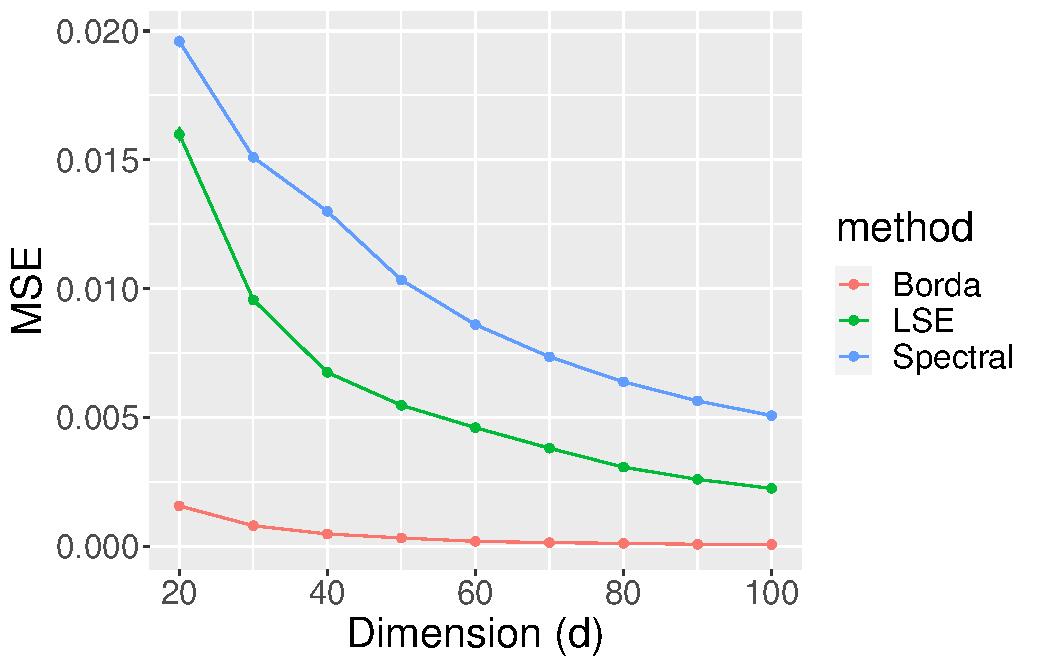
\includegraphics[width = 0.5\textwidth]{figure/model6.pdf}   
    \caption{MSE versus the tensor dimension based on different estimation methods. The true model is defined by the latent function $f(x,y,z)=(x-0.5)^2 +yz$.}
    \label{fig:method2}
\end{figure}

    
 {\bf The general setting. } We realize that the exposition in the original paper may have caused the confusion. Inspired by your comments, we added the following new section in the paper: 
 
 \begin{quote}
{ \color{blue} {\bf Section 5.3 Possible relaxation of monotonicity}\\


%We have shown the success of our Borda count algorithm under extra marginal monotonicity. We refer to $\tF(\alpha,L)\cap \tM(\beta)$ as the monotonic-plus-smooth function class. This class was initially proposed in previous literature of graphons. The work~\citep{chan2014consistent} proposes the Lipschitz monotonic function to facilitate the analysis of sorting-merging algorithm for matrix estimation; their setting is a special case of our Definition 2 with $(\alpha,\beta,m)=(1,1,2)$. Inspired by earlier work, we consider the similar monotonic-plus-smooth function class $\tF(\alpha,L)\cap \tM(\beta)$ under general configuration $\{(\alpha,\beta,m): \alpha>0,\ 0<\beta\min(\alpha,1)\leq 1, \ m\geq 2\}$. Note that the constraint $\beta \min(\alpha, 1) \leq 1$ is due to the natural relationship between joint smoothness and marginal smoothness. \\

We emphasize that our monotonicity assumption should be interpreted \emph{up to permutation} in light of~\eqref{eq:obs}. The permutation relaxes the extent of stringency in the monotonic assumptions. In the univariate case ($m=1$), \emph{every smooth function is monotonic-plus-smooth up to permutations.} In particular, $f\in \tF(1, L)$ implies the existence of permutation $\pi$ such that $(f\circ \pi) \in \tF(1, L)\cap \tB(1)$. The monotonicity comes for free in this case, because the descending sorting, as a permutation, does not deteriorate the 1-d smoothness. For general order~$m$, the monotonicity imposes moderate constraints on the marginal structure. We provide two examples to illustrate flexibility allowed in our models.  \\
  
  
  \begin{example}[Free monotonicity inherited from smoothness]\label{ex:free}Consider a quadratic function $f(x,y,z)=(x-0.5)^2+yz$. Although the function $f$ is non-monotonic, we can show that $f$ is nearly monotonic-plus-smooth up to permutations; i.e., $f$ can be identified by $\bar f\circ \pi$ for some permutation $\pi$ and $\bar f \in \tF(\alpha,L)\cap \tB(\beta)$ up to a negligible perturbation. See appendix~\ref{sec:ex} for the expression of $(\pi, \bar f)$. Therefore, our Borta count algorithm is applicable to $f$.  
 \end{example}
 
  \begin{example}[Decomposable monotonicity] Let $R\in\mathbb{N}_{+}$ be a constant, and $\{g_{r,i}(\cdot) \colon[0,1]\to \bbR\}$ be a set of 1-d smooth functions for $(r,i)\in[R]\times [m]$. Then, all decomposable smooth functions of the form 
  \[
  f(x_1,\ldots,x_m)=\sum_{r\in[R]}g_{r,1}(x_1)\cdots g_{r,m}(x_m),
  \]
are monotonic-plus-smooth up to permutations. In particular, low-rank tensors with smooth factors are also monotonic-plus-smooth up to permutations.
\end{example}
}
 \end{quote}


\item \textit{
    The model is 1-dimensional latent space model. All nodes are embedded into the interval of $[0, 1]$. It is an easier case than a general latent space model where each node is embedded into a $K$-dimensional latent space. Although the block model is a special case of the current model, the current model does not include common variants of block models, such as those with mixed memberships (Jin et al., 2017).
    In the block model, we can encode the community labels by either a $K$-dimensional 0-1 vector $z_i$ or a value $t_i \in \{1, 2, \ldots , K \}$. In the second representation, the latent variables are in dimension 1. However, in a model with mixed membership, only the first representation is possible. The latent variables are in dimension $K$, so finding the latent space is much more than finding an unknown permutation. }
    
    \textbf{Response:} This is an excellent point! In fact, we have been considering the same extension while this paper was in submission. 
The extension from the block model to the mixed membership model is analogous to the extension from 1-dimensional latent space model to general dimensional latent model. 
    This generalization extends the latent permutation $\pi\in\Pi(d,d)$ to the set of latent vectors $\mv_i\in[0,1]^s$.
    
Our parallel work~\citep{lee2023statistical} considers the general dimensional latent variable model similar to reviewer's suggestion. 
  The work~\citep{lee2023statistical} assumes the latent function $f\colon[0,1]^{s}\times\cdots\times[0,1]^{s}\rightarrow \mathbb{R}$ such that
    \begin{align}\label{eq:LVM2}
    \Theta(i_1,\ldots,i_m) = f(\ma^{(1)}_{i_1},\ldots,\ma^{(m)}_{i_m}), \text{ for all } (i_1,\ldots,i_m)\in[d_1]\times\cdots\times [d_m].
\end{align}
where each $a^{(k)}_{i_k}$ is an $s$-dimensional vector with a general $s\geq 1$. In this model, the role of unknown permutation in our paper is extended to the role of unknown latent vectors in~\eqref{eq:LVM2}. However, we find that this extension is not free. We need a stronger assumption than our $\alpha$-smoothness condition for the theoretical analysis. Specifically, we need a new class called \emph{analytic functions} such that
    \begin{align}\label{eq:analytic}
    \sup_{\ma_k\in\mathbb{R}^s, \|\ma_k\|_{\infty}=1, k\in[m]}\left|{\partial^{|\kappa|} f(\ma_1,\ldots,\ma_m)\over \partial(\ma_1,\ma_2,\ldots,\ma_m)^{\kappa}}\right|\leq L^{|\kappa|}\kappa!,\quad \text{for all multi-indices } \kappa\in\bbN^m. 
\end{align}
The analytic function class can be roughly viewed as $\infty$-smoothness plus some extra technical assumptions. The stronger assumption is the price one has to pay for more general model. 

Compared to this current paper, the analysis of analytic functions uses different techniques and yields new results of its own.  For this reason, we decide to not include the extension in current paper. We refer the reviewer to~\citep{lee2023statistical} if interested. 

We have added the above discussion to the revised paper. 
    
    
    \item \textit{
    I suggest that the authors do not over-claim the broadness of the current model and make a careful edit of Section 1.2. The current writing hides the “dimension-1 embedding” nature of the current model and gives readers the wrong impression that the current model is broader than the usual low-rank models.
    }
    
    \textbf{Response:} Thank you for the suggestion. We have added the clarification in Section 1.2. 
    
   \begin{quote}
   {\color{blue}...We emphasize that our permuted smooth tensor model does not necessarily include low-rank model. Compared to low-rank models, we utilize a different measure of \emph{model complexity}.
When the underlying signal is precisely low-rank, then rank might be a reasonable measure for model complexity. However, if the underlying signal is high rank but has certain shape structure, then our nonparametric approach may better capture the intrinsic model complexity.... }
  \end{quote}
    
    We also have added the following paragraph in Section 7:
    \begin{quote}
   { \color{blue}
One limitation of our model is that we consider the 1-dimensional latent space embedding. %The permutation serves as the role of pure membership as in block models. 
The extension from1-dimensional latent space model to general dimensional latent model is analogous to the extension from the block model to the mixed membership model. Our parallel work~\citep{lee2023statistical} considers the general dimensional latent variable model, by assuming  a set of $s$-dimensional vectors $\ma^{(k)}_{i_k}\in\mathbb{R}^s$ with $s\geq 1$ and a latent function $f\colon[0,1]^{s}\times\cdots\times[0,1]^{s}\rightarrow \mathbb{R}$ such that
    \begin{align}\label{eq:LVM2}
    \Theta(i_1,\ldots,i_m) = f(\ma^{(1)}_{i_1},\ldots,\ma^{(m)}_{i_m}), \text{ for all } (i_1,\ldots,i_m)\in[d_1]\times\cdots\times [d_m].
\end{align}
This generalization extends the latent permutation $\pi\in\Pi(d,d)$ to the set of latent vectors in $[0,1]^s$. However, we find that this extension is not free. We need a stronger analytic function class with $\infty$-smoothness for the theoretical analysis. Compared to this current paper, the analysis of analytic functions uses different techniques and yields new results of its own. We refer readers to~\cite{lee2023statistical} for independent interest. }
  \end{quote}
    

    
    
        
    \item \textit{The comparison could be unfair, if other papers did give some polynomial-time algorithms. I suggest the authors to spend more efforts reviewing the algorithms in other papers and discuss whether those algorithms are applicable to the current settings.}
    
    \textbf{Response:} Thank you for the comments. 
    Based on your comments, we added two new results. 
    
 {\bf $-$ In theory,} we have added a new Theorem 3 to show the \emph{non-existence} of polynomial-time algorithm in the general setting. See {\bf pages 1-7 of this response letter, Response to Major comments Summarized by Editor}.  
  
{\bf $-$ In simulation,} we have added more algorithms for comparison. Specifically, we consider:
\begin{itemize}
     \item  Spectral method ({\bf \small Spectral})~\citep{xu2018rates} that performs universal singular value thresholding~\citep{chatterjee2015matrix} on the unfolded tensor.
     \item Least-squares estimation ({\bf \small LSE}) \citep{gao2015rate} which solves the optimization problem \eqref{eq:lseopt} with constant block approximation ($\ell=0$) based on spectral $k$-means. We extend the matrix-based biclustering algorithm to higher-order tensors~\citep{han2022exact}. 
     \item Least-squares estimation ({\bf \small BAL}) \citep{balasubramanian2021nonparametric} which solves the optimization problem \eqref{eq:lseopt} with constant block approximation.
     \item {\color{blue}Cluster+poly$\ell$ algorithm (suggested by the reviewer in \#7) which performs clustering first and then polynomial approximation within clusters.}
 \end{itemize}
The results are provided in the new Figure R2 in this letter. {\bf The comparison is summarized in our response to \#7.} 
    
    
    
    
    \item \textit{In the case of monotonicity, it looks very promising that the rate is faster than Pananjady and Samworth (2022), but the assumptions are different. The rate achieved by Borda count assumes infinite smoothness, which was not assumed in Pananjady and Samworth (2022). The table needs more explanations in the caption, not to mislead the readers.}
    
    
    \textbf{Response:} Thank you for the comments. We update the table accordingly as below; the added parts are highlighted in blue. 
    
 \begin{table*}[h!]
    \centering
    \resizebox{\textwidth}{!}{%
    \begin{tabular}{c|@{\hskip4pt}c@{\hskip5pt}c@{\hskip4pt}c@{\hskip5pt}c@{\hskip4pt}c@{\hskip5pt}c@{\hskip4pt}c@{\hskip5pt}c@{\hskip5pt}c}
    & \citet{pananjady2022isotonic}&  \citet{balasubramanian2021nonparametric}&  \citet{li2019nearest}&\textbf{Ours} (MLE) & \textbf{Ours} (Borda count)\\
    \hline
       Model structure& \color{blue}monotonic & Lipschitz & Lipschitz &  \color{blue}$\alpha$-smooth  & \color{blue}$\alpha$-smooth \& monotonic\\
             Fixed grid design & $\surd$ &$\times$ & $\times$ & $\times$& $\surd$\\
     \vdots&\vdots&\vdots&\vdots&\vdots&\vdots\\
       (e.g., rate when $(m,\alpha)=(3,1)$) & $d^{-1}$& $d^{-6/5}$ & $d^{-1}$ & $d^{-6/5}$ & $d^{-6/5}$\\
          Minimax optimality& $\surd$  & $\times$ & $\times$ & $\surd$ & $-*$  \\
     Polynomial algorithm& $\surd$ &$\times$ & $\surd$ & $\times$& $\surd$ 
    \end{tabular}
    }
    \caption{Comparison of our results with previous work. \color{blue}For simplicity, we omit the log term in the rate. $^{*}$The optimality is achieved under extra Lipchitz monotonicity conditions. Our method allows arbitrary smoothness level $\alpha>0$; see Sections 3-4 for details.}
 \label{tab:comp}
\end{table*}


    \item \textit{Clustering + blockwise polynomial approximation. In the simulations, LSE and BAL first perform clustering and then use constant block approximation. A natural question is what happens if one uses clustering followed by polynomial block approximation. Can the authors add such results into the simulations?
    This is also related to my Point 2. Can this approach replace the Borda count algorithm to produce a polynomial-time algorithm in the case of no monotonicity?
}
  
   \textbf{Response:}
   Thank you for the suggestion. We have added the new algorithm (denoted as cluster + poly$\ell$ algorithm) based on the reviewer's comments. 
The following new result is added to the Appendix~\ref{app:extra}.   
   
   \begin{quote}
   \color{blue}
 ``...We consider another competing algorithm (denoted as cluster + poly$\ell$ algorithm) for comparison. The algorithm performs clustering first and then polynomial approximation within clusters. Since we do not know the permutation, we randomly assign the order of nodes within a block. We perform the simulation using the same setting in Section~\ref{sec:sim}. 
Figure~\ref{fig:method2} shows the comparison among all methods, including the new cluster + poly$\ell$ algorithm for $\ell\in\{1,2,3\}$. Notice that cluster + poly0 algorithm is equivalent to LSE algorithm. The result shows that the cluster + poly$\ell$ algorithms are unstable except Model 3. 

\begin{figure}[ht]
    \centering
    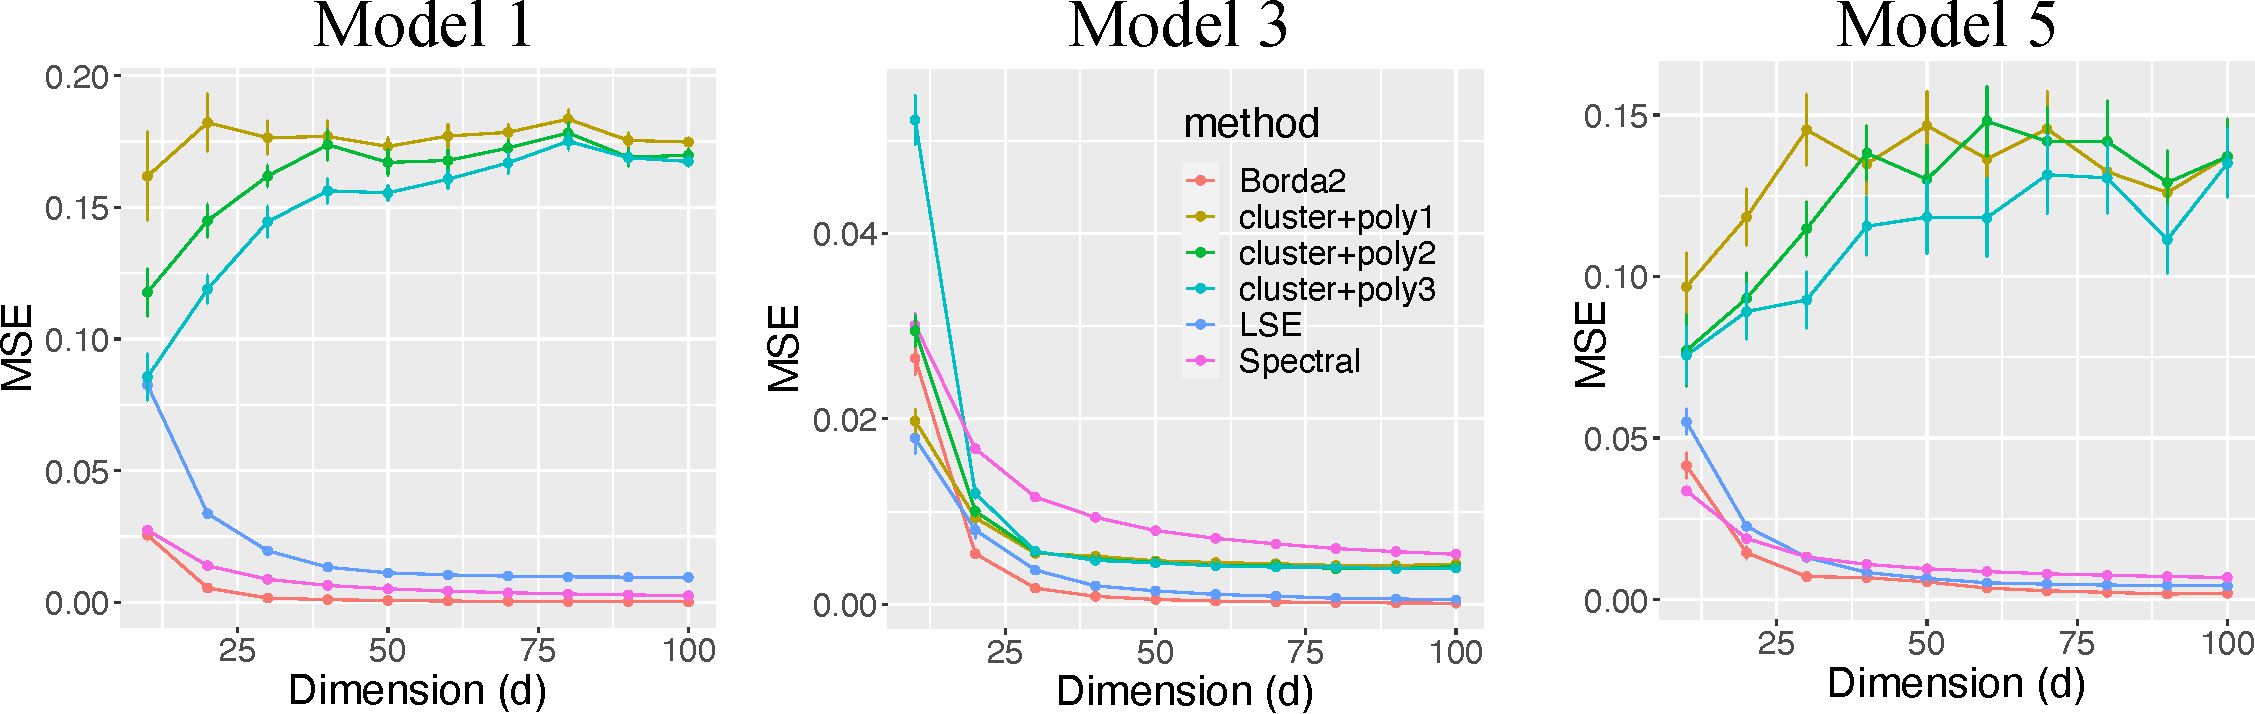
\includegraphics[width = \textwidth]{figure/newalg.pdf}   
    \caption{MSE versus the tensor dimension based on different estimation methods. Columns 1-7 consider the Models 1, 3, and 5 with continuous case in Table~\ref{tb:md} respectively. cluster+poly$\ell$ means polynomial $\ell$-approximation}
    \label{fig:method2}
\end{figure}

   
In fact, we are able to explain the failure of cluster + poly$\ell$ in theory. The two original competing algorithm -- constant block approximation -- does not need the order of nodes. By contrast, the order information is necessary in polynomial approximation in the newly added algorithm. Specifically, the block-$k$ degree-$\ell$ polynomial tensors $\caliB(k,\ell)$ is represented as
\begin{align}\label{eq:polynomial}
    \caliB(k,\ell) = \bigg\{&\tB\in \bbR^{d\times \cdots \times d}\colon \tB(\omega) = \sum_{\Delta\in\tE_k}\text{Poly}_{\ell,\Delta}(\omega)\mathds{1}\{\omega\in\Delta\}\text{ for all } \omega\in[d]^m\bigg\},
\end{align}
where $\text{Poly}_{\ell,\Delta}(\cdot)$ denotes a degree-$\ell$ polynomial function in $\bbR^m$. In the constant block approximation, the polynomial function is   $\text{Poly}_{0,\Delta}(\omega)= \beta^0_{\Delta}$. This implies that an index  $\omega$ does not affect the function estimation. In the linear function approximation,  however,  the polynomial function is $\text{Poly}_{1,\Delta}(\omega)=\langle \boldsymbol{\beta}_{\Delta},\omega\rangle+\beta_{\Delta}^0$ for $\ell=1$, where different index $\omega$ changes the function approximation. Therefore, polynomial approximations with degree greater than 0 require an estimate of the permutation, as in our Borda count algorithm....''
\end{quote}

\end{enumerate}




\bibliographystyle{Chicago.bst}
\bibliography{tensor_wang}

\end{document}
